\documentclass[]{article}
\usepackage{lmodern}
\usepackage{amssymb,amsmath}
\usepackage{ifxetex,ifluatex}
\usepackage{fixltx2e} % provides \textsubscript
\ifnum 0\ifxetex 1\fi\ifluatex 1\fi=0 % if pdftex
  \usepackage[T1]{fontenc}
  \usepackage[utf8]{inputenc}
\else % if luatex or xelatex
  \ifxetex
    \usepackage{mathspec}
  \else
    \usepackage{fontspec}
  \fi
  \defaultfontfeatures{Ligatures=TeX,Scale=MatchLowercase}
\fi
% use upquote if available, for straight quotes in verbatim environments
\IfFileExists{upquote.sty}{\usepackage{upquote}}{}
% use microtype if available
\IfFileExists{microtype.sty}{%
\usepackage{microtype}
\UseMicrotypeSet[protrusion]{basicmath} % disable protrusion for tt fonts
}{}
\usepackage[margin=1in]{geometry}
\usepackage{hyperref}
\hypersetup{unicode=true,
            pdfborder={0 0 0},
            breaklinks=true}
\urlstyle{same}  % don't use monospace font for urls
\usepackage{color}
\usepackage{fancyvrb}
\newcommand{\VerbBar}{|}
\newcommand{\VERB}{\Verb[commandchars=\\\{\}]}
\DefineVerbatimEnvironment{Highlighting}{Verbatim}{commandchars=\\\{\}}
% Add ',fontsize=\small' for more characters per line
\usepackage{framed}
\definecolor{shadecolor}{RGB}{248,248,248}
\newenvironment{Shaded}{\begin{snugshade}}{\end{snugshade}}
\newcommand{\KeywordTok}[1]{\textcolor[rgb]{0.13,0.29,0.53}{\textbf{#1}}}
\newcommand{\DataTypeTok}[1]{\textcolor[rgb]{0.13,0.29,0.53}{#1}}
\newcommand{\DecValTok}[1]{\textcolor[rgb]{0.00,0.00,0.81}{#1}}
\newcommand{\BaseNTok}[1]{\textcolor[rgb]{0.00,0.00,0.81}{#1}}
\newcommand{\FloatTok}[1]{\textcolor[rgb]{0.00,0.00,0.81}{#1}}
\newcommand{\ConstantTok}[1]{\textcolor[rgb]{0.00,0.00,0.00}{#1}}
\newcommand{\CharTok}[1]{\textcolor[rgb]{0.31,0.60,0.02}{#1}}
\newcommand{\SpecialCharTok}[1]{\textcolor[rgb]{0.00,0.00,0.00}{#1}}
\newcommand{\StringTok}[1]{\textcolor[rgb]{0.31,0.60,0.02}{#1}}
\newcommand{\VerbatimStringTok}[1]{\textcolor[rgb]{0.31,0.60,0.02}{#1}}
\newcommand{\SpecialStringTok}[1]{\textcolor[rgb]{0.31,0.60,0.02}{#1}}
\newcommand{\ImportTok}[1]{#1}
\newcommand{\CommentTok}[1]{\textcolor[rgb]{0.56,0.35,0.01}{\textit{#1}}}
\newcommand{\DocumentationTok}[1]{\textcolor[rgb]{0.56,0.35,0.01}{\textbf{\textit{#1}}}}
\newcommand{\AnnotationTok}[1]{\textcolor[rgb]{0.56,0.35,0.01}{\textbf{\textit{#1}}}}
\newcommand{\CommentVarTok}[1]{\textcolor[rgb]{0.56,0.35,0.01}{\textbf{\textit{#1}}}}
\newcommand{\OtherTok}[1]{\textcolor[rgb]{0.56,0.35,0.01}{#1}}
\newcommand{\FunctionTok}[1]{\textcolor[rgb]{0.00,0.00,0.00}{#1}}
\newcommand{\VariableTok}[1]{\textcolor[rgb]{0.00,0.00,0.00}{#1}}
\newcommand{\ControlFlowTok}[1]{\textcolor[rgb]{0.13,0.29,0.53}{\textbf{#1}}}
\newcommand{\OperatorTok}[1]{\textcolor[rgb]{0.81,0.36,0.00}{\textbf{#1}}}
\newcommand{\BuiltInTok}[1]{#1}
\newcommand{\ExtensionTok}[1]{#1}
\newcommand{\PreprocessorTok}[1]{\textcolor[rgb]{0.56,0.35,0.01}{\textit{#1}}}
\newcommand{\AttributeTok}[1]{\textcolor[rgb]{0.77,0.63,0.00}{#1}}
\newcommand{\RegionMarkerTok}[1]{#1}
\newcommand{\InformationTok}[1]{\textcolor[rgb]{0.56,0.35,0.01}{\textbf{\textit{#1}}}}
\newcommand{\WarningTok}[1]{\textcolor[rgb]{0.56,0.35,0.01}{\textbf{\textit{#1}}}}
\newcommand{\AlertTok}[1]{\textcolor[rgb]{0.94,0.16,0.16}{#1}}
\newcommand{\ErrorTok}[1]{\textcolor[rgb]{0.64,0.00,0.00}{\textbf{#1}}}
\newcommand{\NormalTok}[1]{#1}
\usepackage{longtable,booktabs}
\usepackage{graphicx,grffile}
\makeatletter
\def\maxwidth{\ifdim\Gin@nat@width>\linewidth\linewidth\else\Gin@nat@width\fi}
\def\maxheight{\ifdim\Gin@nat@height>\textheight\textheight\else\Gin@nat@height\fi}
\makeatother
% Scale images if necessary, so that they will not overflow the page
% margins by default, and it is still possible to overwrite the defaults
% using explicit options in \includegraphics[width, height, ...]{}
\setkeys{Gin}{width=\maxwidth,height=\maxheight,keepaspectratio}
\IfFileExists{parskip.sty}{%
\usepackage{parskip}
}{% else
\setlength{\parindent}{0pt}
\setlength{\parskip}{6pt plus 2pt minus 1pt}
}
\setlength{\emergencystretch}{3em}  % prevent overfull lines
\providecommand{\tightlist}{%
  \setlength{\itemsep}{0pt}\setlength{\parskip}{0pt}}
\setcounter{secnumdepth}{0}
% Redefines (sub)paragraphs to behave more like sections
\ifx\paragraph\undefined\else
\let\oldparagraph\paragraph
\renewcommand{\paragraph}[1]{\oldparagraph{#1}\mbox{}}
\fi
\ifx\subparagraph\undefined\else
\let\oldsubparagraph\subparagraph
\renewcommand{\subparagraph}[1]{\oldsubparagraph{#1}\mbox{}}
\fi

%%% Use protect on footnotes to avoid problems with footnotes in titles
\let\rmarkdownfootnote\footnote%
\def\footnote{\protect\rmarkdownfootnote}

%%% Change title format to be more compact
\usepackage{titling}

% Create subtitle command for use in maketitle
\newcommand{\subtitle}[1]{
  \posttitle{
    \begin{center}\large#1\end{center}
    }
}

\setlength{\droptitle}{-2em}

  \title{}
    \pretitle{\vspace{\droptitle}}
  \posttitle{}
    \author{}
    \preauthor{}\postauthor{}
    \date{}
    \predate{}\postdate{}
  

\begin{document}

Some normal text.

\begin{verbatim}
## [1] "table of lithic types"
\end{verbatim}

\begin{longtable}[]{@{}lll@{}}
\toprule
type & count & proportion\tabularnewline
\midrule
\endhead
flake\_ids & 1199 & 0.541\tabularnewline
core\_ids & 249 & 0.112\tabularnewline
debris\_ids & 769 & 0.347\tabularnewline
total & 2217 & 1\tabularnewline
\bottomrule
\end{longtable}

\begin{verbatim}
## [1] "tables for raw materials of the assemblage"
\end{verbatim}

\begin{longtable}[]{@{}lrrrrrr@{}}
\toprule
category & chert & limestone & basalt & quartz & sandstone &
total\tabularnewline
\midrule
\endhead
flake & 932 & 249 & 11 & 2 & 5 & 1199\tabularnewline
core & 208 & 38 & 2 & 0 & 0 & 248\tabularnewline
debris & 569 & 190 & 8 & 1 & 1 & 769\tabularnewline
retouched pieces & 767 & 201 & 11 & 1 & 4 & 984\tabularnewline
backed knife & 6 & 2 & 0 & 0 & 0 & 8\tabularnewline
bec & 6 & 1 & 0 & 0 & 0 & 7\tabularnewline
borer & 52 & 17 & 0 & 0 & 0 & 69\tabularnewline
BUR & 4 & 1 & 0 & 0 & 0 & 5\tabularnewline
chopper & 0 & 0 & 1 & 0 & 0 & 1\tabularnewline
cleaver & 1 & 0 & 0 & 0 & 0 & 1\tabularnewline
Denticular & 54 & 21 & 1 & 0 & 1 & 77\tabularnewline
Endscraper & 32 & 6 & 0 & 0 & 0 & 38\tabularnewline
Point & 24 & 5 & 0 & 0 & 0 & 29\tabularnewline
scraper & 486 & 130 & 7 & 1 & 3 & 627\tabularnewline
nature backed & 4 & 2 & 0 & 0 & 0 & 6\tabularnewline
notch & 65 & 12 & 2 & 0 & 0 & 79\tabularnewline
tanged point & 9 & 1 & 0 & 0 & 0 & 10\tabularnewline
\bottomrule
\end{longtable}

\begin{verbatim}
## [1] "proportion tables for raw materials of the assemblage"
\end{verbatim}

\begin{longtable}[]{@{}lrrrrrr@{}}
\toprule
category & chert & limestone & basalt & quartz & sandstone &
total\tabularnewline
\midrule
\endhead
flake & 77.7 & 20.8 & 0.9 & 0.2 & 0.4 & 100\tabularnewline
core & 83.9 & 15.3 & 0.8 & 0.0 & 0.0 & 100\tabularnewline
debris & 74.0 & 24.7 & 1.0 & 0.1 & 0.1 & 100\tabularnewline
retouched pieces & 77.9 & 20.4 & 1.1 & 0.1 & 0.4 & 100\tabularnewline
backed knife & 75.0 & 25.0 & 0.0 & 0.0 & 0.0 & 100\tabularnewline
bec & 85.7 & 14.3 & 0.0 & 0.0 & 0.0 & 100\tabularnewline
borer & 75.4 & 24.6 & 0.0 & 0.0 & 0.0 & 100\tabularnewline
BUR & 80.0 & 20.0 & 0.0 & 0.0 & 0.0 & 100\tabularnewline
chopper & 0.0 & 0.0 & 100.0 & 0.0 & 0.0 & 100\tabularnewline
cleaver & 100.0 & 0.0 & 0.0 & 0.0 & 0.0 & 100\tabularnewline
Denticular & 70.1 & 27.3 & 1.3 & 0.0 & 1.3 & 100\tabularnewline
Endscraper & 84.2 & 15.8 & 0.0 & 0.0 & 0.0 & 100\tabularnewline
Point & 82.8 & 17.2 & 0.0 & 0.0 & 0.0 & 100\tabularnewline
scraper & 77.5 & 20.7 & 1.1 & 0.2 & 0.5 & 100\tabularnewline
nature backed & 66.7 & 33.3 & 0.0 & 0.0 & 0.0 & 100\tabularnewline
notch & 82.3 & 15.2 & 2.5 & 0.0 & 0.0 & 100\tabularnewline
tanged point & 90.0 & 10.0 & 0.0 & 0.0 & 0.0 & 100\tabularnewline
\bottomrule
\end{longtable}

\begin{verbatim}
## [1] "summary of core attributes"
\end{verbatim}

\begin{longtable}[]{@{}lrrrrrrrrrrrr@{}}
\toprule
& length & max\_dimension & medial\_width & distal\_width & thickness &
distal\_thickness & mass & platform & platform\_width &
platform\_thickness & scar\_number & cortex\_percentage\tabularnewline
\midrule
\endhead
mean & 47.2 & 75.1 & 58.0 & 49.2 & 51.8 & 38.7 & 198.9 & 1.5 & 50.9 &
43.7 & 2.9 & 14.5\tabularnewline
sd & 20.2 & 21.6 & 21.2 & 21.5 & 29.6 & 17.1 & 166.8 & 0.8 & 20.0 & 19.8
& 2.0 & 19.4\tabularnewline
CV & 0.4 & 0.3 & 0.4 & 0.4 & 0.6 & 0.4 & 0.8 & 0.5 & 0.4 & 0.5 & 0.7 &
1.3\tabularnewline
25\% & 33.0 & 63.0 & 43.0 & 35.2 & 38.2 & 27.2 & 100.2 & 1.0 & 37.0 &
30.2 & 1.2 & 0.0\tabularnewline
50\% & 43.5 & 72.0 & 55.0 & 45.0 & 47.0 & 37.0 & 149.5 & 1.0 & 50.0 &
40.0 & 2.0 & 7.5\tabularnewline
75\% & 57.8 & 83.8 & 68.0 & 60.6 & 60.8 & 48.0 & 243.0 & 2.0 & 61.8 &
51.9 & 4.0 & 20.0\tabularnewline
\bottomrule
\end{longtable}

\begin{verbatim}
## [1] "cortex proportion of cores"
\end{verbatim}

\includegraphics{for_paper_ii_files/figure-latex/unnamed-chunk-2-1.pdf}

We will try univariate clustering for flake mass:

\begin{verbatim}
## [1] "flake grouping result according to mass"
\end{verbatim}

\includegraphics{for_paper_ii_files/figure-latex/unnamed-chunk-3-1.pdf}

\begin{verbatim}
##  [1] "crest"          "DBD"            "flake"          "KBW"           
##  [5] "leva"           "LVF"            "LVF_?"          "ret"           
##  [9] "ret brk"        "ret leva?"      "ret pro-lepoin" "tablet"        
## [13] "blade"          "leva?"          "blade brk?"     "BUR"           
## [17] "FACETED"        "flake brk"      "LVFB"           "LVT"           
## [21] "proximal"       NA
\end{verbatim}

\begin{verbatim}
## [1] "compare the mass of Leva and non-leva flakes"
\end{verbatim}

\includegraphics{for_paper_ii_files/figure-latex/unnamed-chunk-4-1.pdf}

\begin{verbatim}
## [1] "t-test to see if it is statistically significant?"
\end{verbatim}

\begin{verbatim}
## 
##  Welch Two Sample t-test
## 
## data:  mass by L
## t = -1.9714, df = 64.674, p-value = 0.05296
## alternative hypothesis: true difference in means is not equal to 0
## 95 percent confidence interval:
##  -28.6440377   0.1870471
## sample estimates:
## mean in group L mean in group N 
##        39.28571        53.51421
\end{verbatim}

\begin{verbatim}
## [1] "variation of thickness for all flakes (red = 25%max_dim,green = 50%max,blue=75%max"
\end{verbatim}

\includegraphics{for_paper_ii_files/figure-latex/unnamed-chunk-4-2.pdf}

\begin{verbatim}
## [1] "compare thickness of leva and non-leva (red = 25%max_dim, \n      green = 50%max, blue=75%max"
\end{verbatim}

\includegraphics{for_paper_ii_files/figure-latex/unnamed-chunk-4-3.pdf}

\begin{verbatim}
## [1] "summary of cv for thickness and width for leva and non-leva flakes"
\end{verbatim}

\begin{verbatim}
## # A tibble: 2 x 8
##   L     cv_25_thick cv_50_thick cv_75_thick cv_25_width cv_50_width
##   <chr>       <dbl>       <dbl>       <dbl>       <dbl>       <dbl>
## 1 L            40.2        40.0        42.7        38.3        36.0
## 2 N            48.8        44.7        46.0        79.3        40.6
## # ... with 2 more variables: cv_75_width <dbl>, n <int>
\end{verbatim}

The following are results for cores

\begin{verbatim}
## [1] "summary for core geometry"
\end{verbatim}

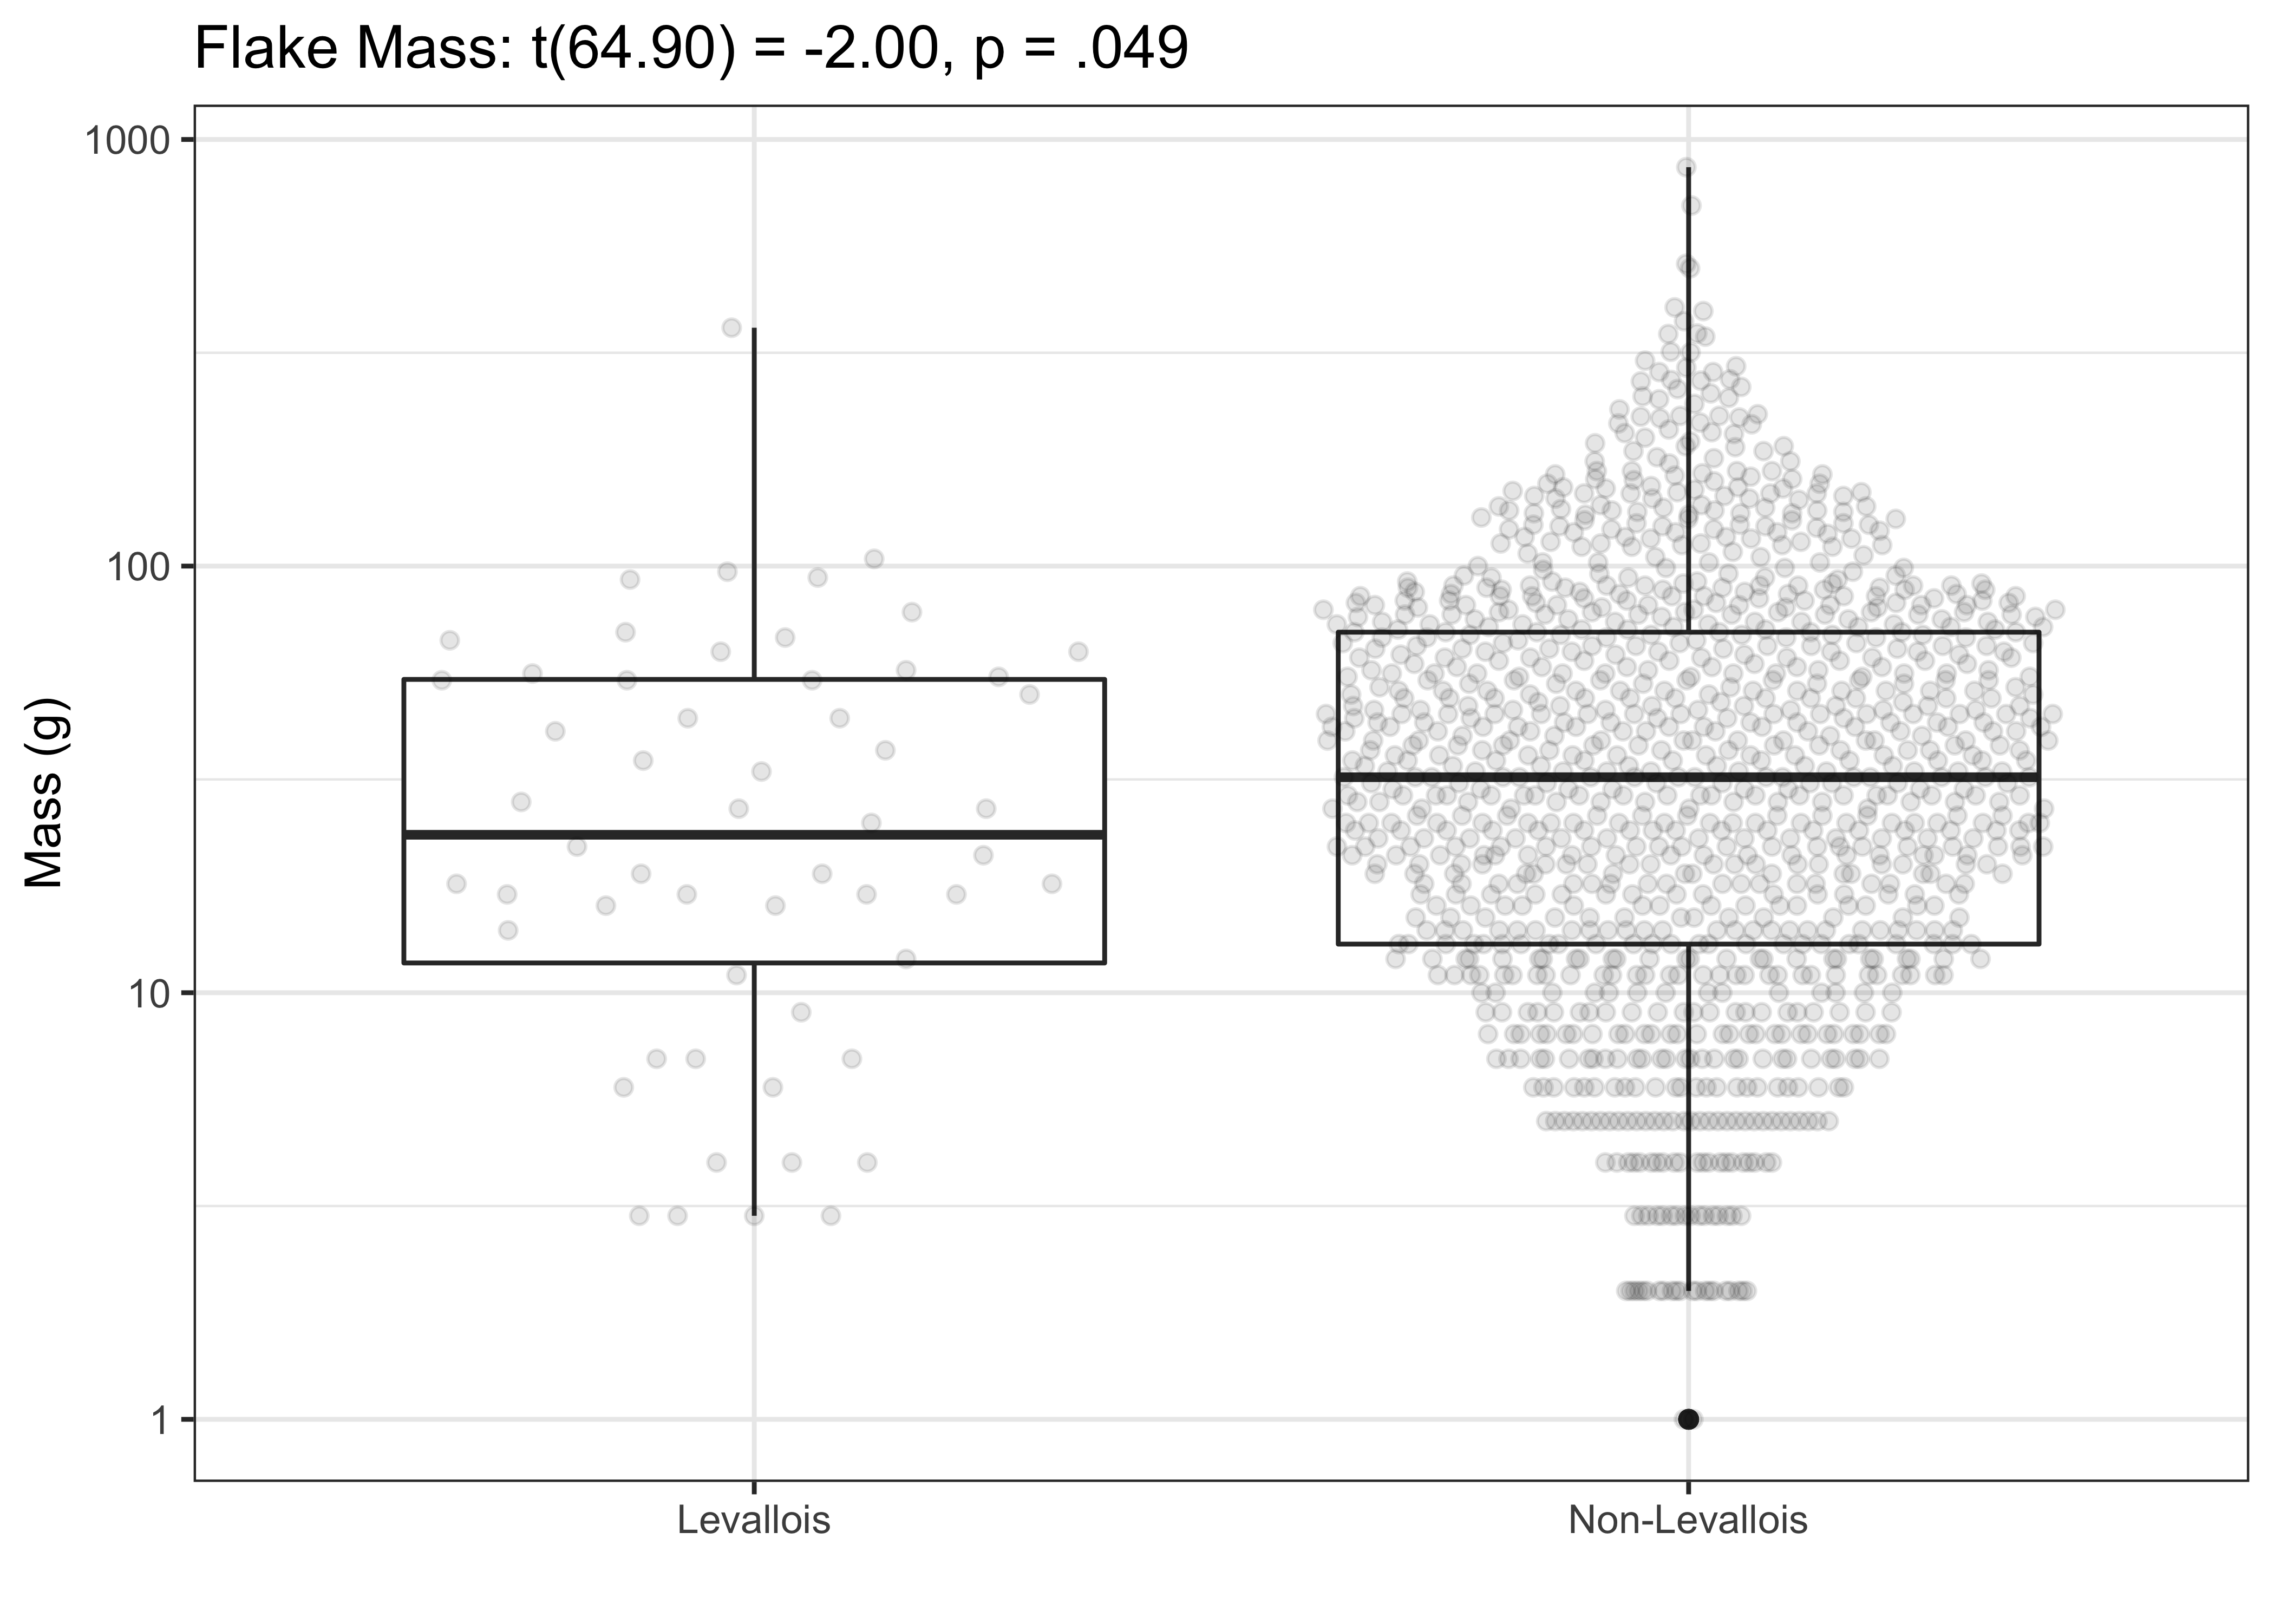
\includegraphics{for_paper_ii_files/figure-latex/unnamed-chunk-5-1.pdf}

\begin{verbatim}
## 
##   circle   column    conic    cubic  end,scp iregular   wedged 
##     0.61     6.71     9.76     0.61     0.61    80.49     1.22
\end{verbatim}

\begin{verbatim}
## [1] "summary for core platform"
\end{verbatim}

\includegraphics{for_paper_ii_files/figure-latex/unnamed-chunk-5-2.pdf}

\begin{verbatim}
## 
##     1     2     3     4     5    36 
## 60.49 27.16  6.17  4.94  0.62  0.62
\end{verbatim}

\begin{verbatim}
## [1] "summary for core platform preparation"
\end{verbatim}

\includegraphics{for_paper_ii_files/figure-latex/unnamed-chunk-5-3.pdf}

\begin{verbatim}
## 
##  cortex   dehid faceted       n    over   plain   plane 
##    3.38    0.68   18.24    6.76   15.54   54.05    1.35
\end{verbatim}

\begin{verbatim}
## [1] "summary for core rotations"
\end{verbatim}

\includegraphics{for_paper_ii_files/figure-latex/unnamed-chunk-5-4.pdf}

\begin{verbatim}
## 
##     0     1     2     3     4     5 
##  8.05 59.73 22.15  6.04  2.68  1.34
\end{verbatim}

\begin{verbatim}
## [1] "summary for core reduction type"
\end{verbatim}

\includegraphics{for_paper_ii_files/figure-latex/unnamed-chunk-5-5.pdf}

\begin{verbatim}
## 
## <U+7A84><U+9762><U+77F3><U+6838>           BIFACIAL      BIFACIAL CORE 
##               0.40               1.21               2.42 
##         blade core             blade?               core 
##               4.84               1.21               0.40 
##               disc             double               HMSF 
##               3.63              12.50               2.82 
##           KBW CORE             KBW/TF               leva 
##               0.81               3.23               0.40 
##                LVC            LVC/DIS   LVC?HMSF? DOUBLE 
##               4.44               0.40               0.40 
## LVMC(LV MIDDLE)/TF              multp         MULTP CORE 
##               0.40               5.65               0.40 
##             pebble          pre leva?             single 
##               0.40               0.40              31.05 
##        SINGLE CORE           spheroid                 TF 
##               0.81               0.40              21.37
\end{verbatim}

\begin{verbatim}
## [1] "summary of core scar number"
\end{verbatim}

\includegraphics{for_paper_ii_files/figure-latex/unnamed-chunk-5-6.pdf}

\begin{verbatim}
## 
##     1     2     3     4     5     6     7     8     9    10    14 
## 24.84 24.22 16.77 16.15  9.32  4.97  1.24  0.62  0.62  0.62  0.62
\end{verbatim}

The following results are for flakes

\begin{verbatim}
## [1] "table for flake attributes"
\end{verbatim}

\begin{longtable}[]{@{}lrrrrrrrrrrrrrrr@{}}
\toprule
& length & max\_dimension & oriented\_width & Width\_25\%max &
Width\_50\%max & Width\_75\%max & oriented\_thickness &
Thickness\_25\%max & Thickness\_50\%max & Thickness\_75\%max & mass &
platform\_width & platform\_thickness & scar\_number &
cortex\_percentage\tabularnewline
\midrule
\endhead
mean & 49.4 & 62.5 & 50.3 & 38.3 & 41.9 & 35.2 & 17.6 & 16.1 & 16.6 &
13.7 & 68.2 & 32.8 & 13.7 & 2.9 & 9.4\tabularnewline
sd & 19.2 & 22.5 & 19.2 & 38.6 & 15.3 & 14.8 & 8.1 & 7.6 & 7.8 & 6.8 &
81.7 & 16.8 & 7.8 & 1.6 & 15.1\tabularnewline
cv & 0.4 & 0.4 & 0.4 & 1.0 & 0.4 & 0.4 & 0.5 & 0.5 & 0.5 & 0.5 & 1.2 &
0.5 & 0.6 & 0.6 & 1.6\tabularnewline
25\% & 35.0 & 48.2 & 36.0 & 26.0 & 30.1 & 25.0 & 11.8 & 10.9 & 11.0 &
9.0 & 18.8 & 19.9 & 8.0 & 2.0 & 0.0\tabularnewline
50\% & 48.0 & 60.0 & 49.0 & 35.0 & 41.0 & 34.0 & 16.0 & 15.0 & 15.0 &
12.6 & 45.5 & 30.9 & 12.0 & 3.0 & 0.0\tabularnewline
75\% & 60.8 & 76.0 & 61.7 & 44.9 & 51.1 & 43.0 & 23.0 & 20.9 & 21.0 &
18.0 & 90.0 & 43.0 & 18.3 & 4.0 & 10.0\tabularnewline
\bottomrule
\end{longtable}

\begin{verbatim}
## [1] "summary for flake type1"
\end{verbatim}

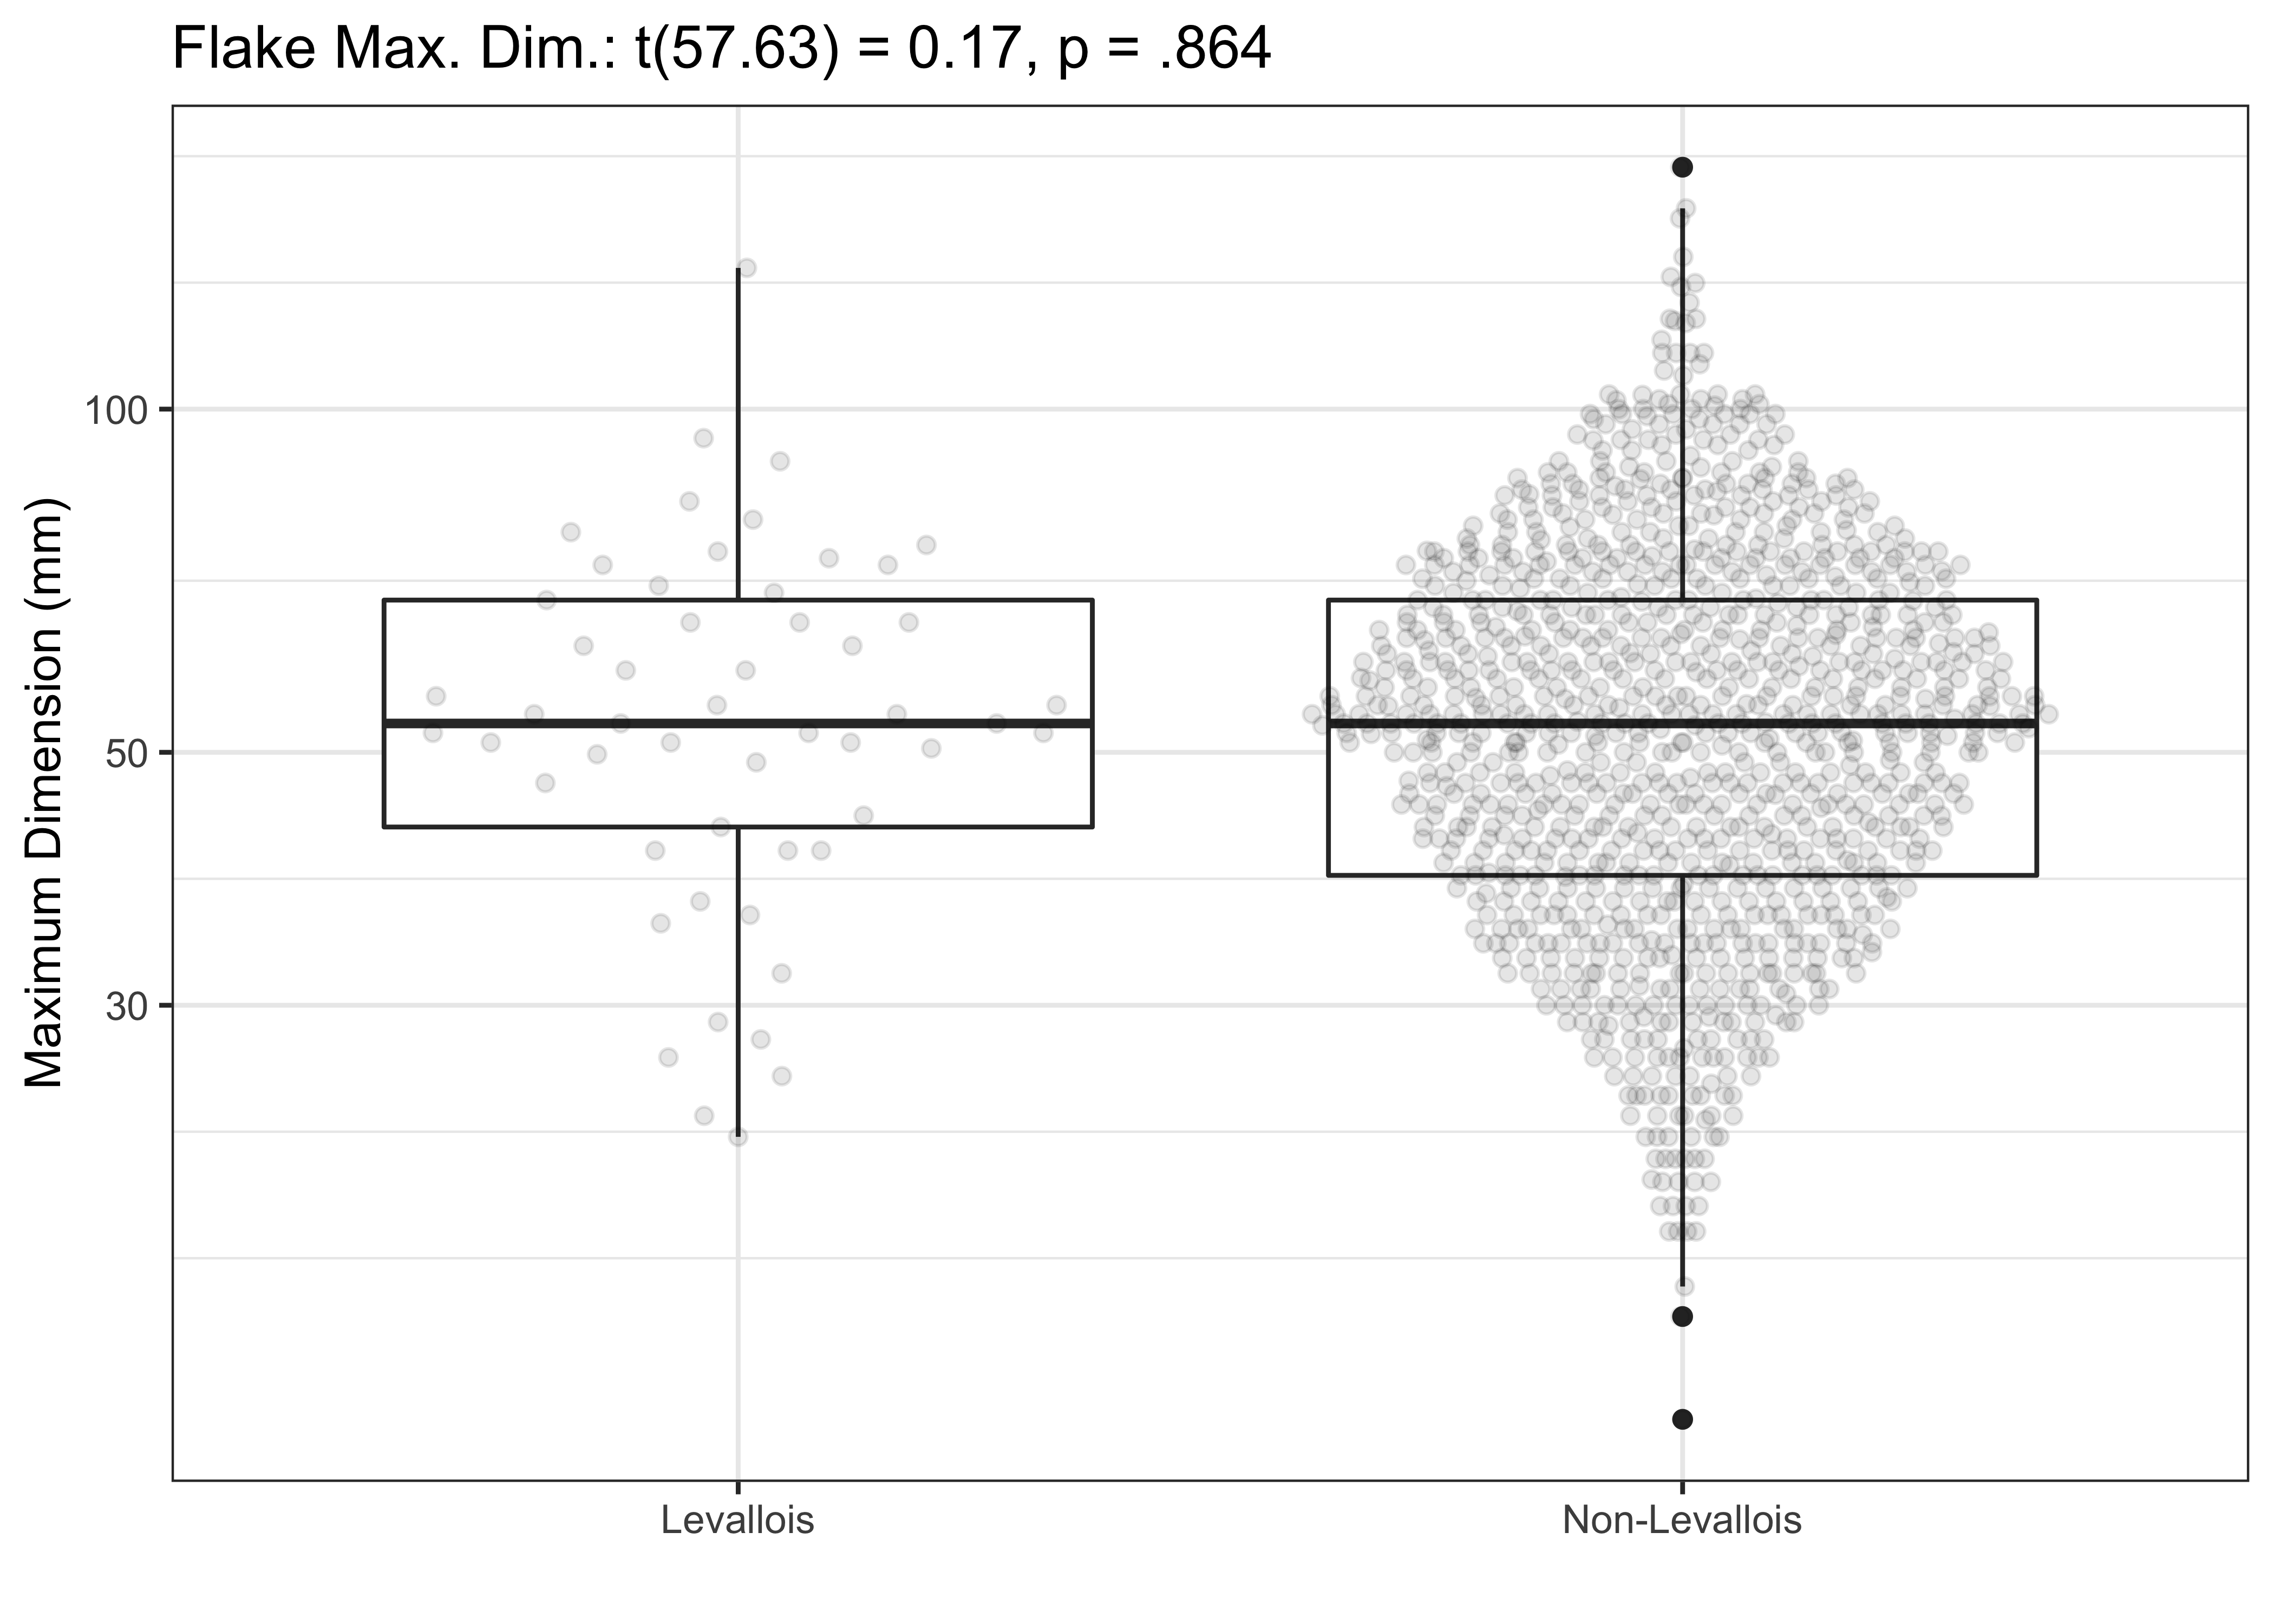
\includegraphics{for_paper_ii_files/figure-latex/unnamed-chunk-6-1.pdf}

\begin{verbatim}
## 
##          blade     blade brk?            BUR          crest            DBD 
##              2              1              1              1             26 
##        FACETED          flake      flake brk            KBW           leva 
##              1            123              2             20             12 
##          leva?            LVF          LVF_?           LVFB            LVT 
##              1             30             21              3              3 
##       proximal            ret        ret brk      ret leva? ret pro-lepoin 
##              1            202            720              5              1 
##         tablet 
##              3
\end{verbatim}

\begin{verbatim}
## 
##          blade     blade brk?            BUR          crest            DBD 
##            0.2            0.1            0.1            0.1            2.2 
##        FACETED          flake      flake brk            KBW           leva 
##            0.1           10.4            0.2            1.7            1.0 
##          leva?            LVF          LVF_?           LVFB            LVT 
##            0.1            2.5            1.8            0.3            0.3 
##       proximal            ret        ret brk      ret leva? ret pro-lepoin 
##            0.1           17.1           61.1            0.4            0.1 
##         tablet 
##            0.3
\end{verbatim}

\begin{verbatim}
## [1] "summary for flake type2"
\end{verbatim}

\includegraphics{for_paper_ii_files/figure-latex/unnamed-chunk-6-2.pdf}

\begin{verbatim}
## 
##       backed knife                bec            bec,scp 
##                  8                  4                  3 
##              blade              borer         borer,dent 
##                  1                 13                  1 
##     borer,dent,scp      borer,end,scp        borer,notch 
##                  2                  1                  2 
##    borer,notch,scp          borer,scp      borer,scp,end 
##                  1                 47                  1 
##         borer,strt                BUR         BUR? CORE? 
##                  1                  3                  1 
##              burin              BURIN            cleaver 
##                  1                  2                  1 
## convergent sidescp                 cp              crest 
##                  1                  1                  1 
##               dent     dent,borer,scp           dent,end 
##                 51                  1                  1 
##         dent,notch           dent,scp           dent/NOT 
##                  2                 20                  1 
##         dent/POINT                end          end,borer 
##                  1                 14                  1 
##      end,borer,scp            end,scp             endscp 
##                  1                 17                  6 
##            kombewa               leva         leva point 
##                  1                  2                  1 
##        leva point?              leva?               moon 
##                  2                  1                  7 
##            NATBACK      nature backed             notcch 
##                  7                  1                  1 
##              notch        notch,borer          notch,end 
##                 61                  2                  2 
##          notch,scp         notch/DENT              point 
##                 21                  1                 22 
##              POINT        point break       point,broken 
##                  1                  1                  1 
##             point?          PSD POINT                scp 
##                  5                  1                606 
##            sidescp        sidescp-cvx             tablet 
##                 20                  1                  1 
##       tablet break               TANG             TANGED 
##                  1                  1                  1 
##       TANGED POINT  TANGED POINT /NOT      tanged point? 
##                  3                  1                  3 
##      TANGED POINT?      THINING POINT         TRANVS SCP 
##                  1                  1                  1
\end{verbatim}

\begin{verbatim}
## 
##       backed knife                bec            bec,scp 
##                0.8                0.4                0.3 
##              blade              borer         borer,dent 
##                0.1                1.3                0.1 
##     borer,dent,scp      borer,end,scp        borer,notch 
##                0.2                0.1                0.2 
##    borer,notch,scp          borer,scp      borer,scp,end 
##                0.1                4.7                0.1 
##         borer,strt                BUR         BUR? CORE? 
##                0.1                0.3                0.1 
##              burin              BURIN            cleaver 
##                0.1                0.2                0.1 
## convergent sidescp                 cp              crest 
##                0.1                0.1                0.1 
##               dent     dent,borer,scp           dent,end 
##                5.1                0.1                0.1 
##         dent,notch           dent,scp           dent/NOT 
##                0.2                2.0                0.1 
##         dent/POINT                end          end,borer 
##                0.1                1.4                0.1 
##      end,borer,scp            end,scp             endscp 
##                0.1                1.7                0.6 
##            kombewa               leva         leva point 
##                0.1                0.2                0.1 
##        leva point?              leva?               moon 
##                0.2                0.1                0.7 
##            NATBACK      nature backed             notcch 
##                0.7                0.1                0.1 
##              notch        notch,borer          notch,end 
##                6.1                0.2                0.2 
##          notch,scp         notch/DENT              point 
##                2.1                0.1                2.2 
##              POINT        point break       point,broken 
##                0.1                0.1                0.1 
##             point?          PSD POINT                scp 
##                0.5                0.1               61.0 
##            sidescp        sidescp-cvx             tablet 
##                2.0                0.1                0.1 
##       tablet break               TANG             TANGED 
##                0.1                0.1                0.1 
##       TANGED POINT  TANGED POINT /NOT      tanged point? 
##                0.3                0.1                0.3 
##      TANGED POINT?      THINING POINT         TRANVS SCP 
##                0.1                0.1                0.1
\end{verbatim}

\begin{verbatim}
## [1] "summary for flake retouch"
\end{verbatim}

\includegraphics{for_paper_ii_files/figure-latex/unnamed-chunk-6-3.pdf}

\begin{verbatim}
## 
##   retouched unretouched 
##         928         258
\end{verbatim}

\begin{verbatim}
## 
##   retouched unretouched 
##        78.2        21.8
\end{verbatim}

\begin{verbatim}
## [1] "summary for flake material"
\end{verbatim}

\includegraphics{for_paper_ii_files/figure-latex/unnamed-chunk-6-4.pdf}

\begin{verbatim}
## [1] "summary for flake platform shape"
\end{verbatim}

\includegraphics{for_paper_ii_files/figure-latex/unnamed-chunk-6-5.pdf}

\begin{verbatim}
## 
##   fusiform   gullwing   iregular quadrangle  rectangle  trapezoid 
##         46         31          1         87          1          4 
##   triangle 
##        136
\end{verbatim}

\begin{verbatim}
## 
##   fusiform   gullwing   iregular quadrangle  rectangle  trapezoid 
##      15.03      10.13       0.33      28.43       0.33       1.31 
##   triangle 
##      44.44
\end{verbatim}

\begin{verbatim}
## [1] "summary for flake platform"
\end{verbatim}

\includegraphics{for_paper_ii_files/figure-latex/unnamed-chunk-6-6.pdf}

\begin{verbatim}
## [1] "number of flakes with distinctive platform = 396"
\end{verbatim}

\begin{verbatim}
## 
##              cotex          dihederal            faceted 
##                 36                 45                 42 
## faceted(LEVA LIKE)           FACETED?              focus 
##                  1                  3                 20 
##               miss              overh              plain 
##                 35                  1                212 
##          RETOUCHED 
##                  1
\end{verbatim}

\begin{verbatim}
## 
##              cotex          dihederal            faceted 
##                9.1               11.4               10.6 
## faceted(LEVA LIKE)           FACETED?              focus 
##                0.3                0.8                5.1 
##               miss              overh              plain 
##                8.8                0.3               53.5 
##          RETOUCHED 
##                0.3
\end{verbatim}

\begin{verbatim}
## [1] "mass of flakes"
\end{verbatim}

\includegraphics{for_paper_ii_files/figure-latex/unnamed-chunk-6-7.pdf}
\includegraphics{for_paper_ii_files/figure-latex/unnamed-chunk-6-8.pdf}

\begin{verbatim}
## [1] "length vs width at 50% max dim"
\end{verbatim}

\includegraphics{for_paper_ii_files/figure-latex/unnamed-chunk-6-9.pdf}

\begin{verbatim}
## [1] "platform shape vs thickness at 50% max dim"
\end{verbatim}

\includegraphics{for_paper_ii_files/figure-latex/unnamed-chunk-6-10.pdf}

\begin{verbatim}
## [1] "mass for retouched and non-retouched flakes"
\end{verbatim}

\includegraphics{for_paper_ii_files/figure-latex/unnamed-chunk-6-11.pdf}

\begin{verbatim}
## [1] "mass for flakes of different raw materials"
\end{verbatim}

\includegraphics{for_paper_ii_files/figure-latex/unnamed-chunk-6-12.pdf}

\begin{verbatim}
## [1] "max dim for all flakes"
\end{verbatim}

\includegraphics{for_paper_ii_files/figure-latex/unnamed-chunk-6-13.pdf}

\begin{verbatim}
## [1] "max dim for all flakes, retouched or not"
\end{verbatim}

\includegraphics{for_paper_ii_files/figure-latex/unnamed-chunk-6-14.pdf}

\begin{verbatim}
## [1] "max dim for all flakes, by raw material"
\end{verbatim}

\includegraphics{for_paper_ii_files/figure-latex/unnamed-chunk-6-15.pdf}

\begin{verbatim}
## [1] "scar counts for all flakes, by raw material"
\end{verbatim}

\includegraphics{for_paper_ii_files/figure-latex/unnamed-chunk-6-16.pdf}
\includegraphics{for_paper_ii_files/figure-latex/unnamed-chunk-6-17.pdf}

\begin{verbatim}
## [1] "facetted platforms"
\end{verbatim}

\begin{verbatim}
## 
##  fac   no 
##   43 1143
\end{verbatim}

\begin{verbatim}
## 
##   fac    no 
##  3.63 96.37
\end{verbatim}

\includegraphics{for_paper_ii_files/figure-latex/unnamed-chunk-6-18.pdf}

\begin{verbatim}
## [1] "cortex proportion of flakes"
\end{verbatim}

\includegraphics{for_paper_ii_files/figure-latex/unnamed-chunk-6-19.pdf}

\begin{verbatim}
## [1] "compare cortex for ret and non-retouched flakes"
\end{verbatim}

\includegraphics{for_paper_ii_files/figure-latex/unnamed-chunk-6-20.pdf}
\includegraphics{for_paper_ii_files/figure-latex/unnamed-chunk-6-21.pdf}

\begin{verbatim}
## [1] "platform shape vs max dim"
\end{verbatim}

\includegraphics{for_paper_ii_files/figure-latex/unnamed-chunk-6-22.pdf}

\begin{verbatim}
## [1] "how many points?"
\end{verbatim}

\begin{verbatim}
## 
## backed  other  point 
##      9   1133     44
\end{verbatim}

\begin{verbatim}
## 
## backed  other  point 
##   0.76  95.53   3.71
\end{verbatim}

Group the flakes according to their

\begin{Shaded}
\begin{Highlighting}[]
\CommentTok{# Look to see if groups exist}

\CommentTok{# by flake size}
\NormalTok{plain_flakes <-}\StringTok{  }\NormalTok{flakes[}\KeywordTok{grepl}\NormalTok{(}\StringTok{"fl"}\NormalTok{, flakes}\OperatorTok{$}\NormalTok{type1), ]}
\NormalTok{d <-}\StringTok{ }\KeywordTok{density}\NormalTok{(}\KeywordTok{na.omit}\NormalTok{(plain_flakes}\OperatorTok{$}\NormalTok{mass)) }\CommentTok{# returns the density data}
\CommentTok{# plot}
\KeywordTok{plot}\NormalTok{(d)}
\end{Highlighting}
\end{Shaded}

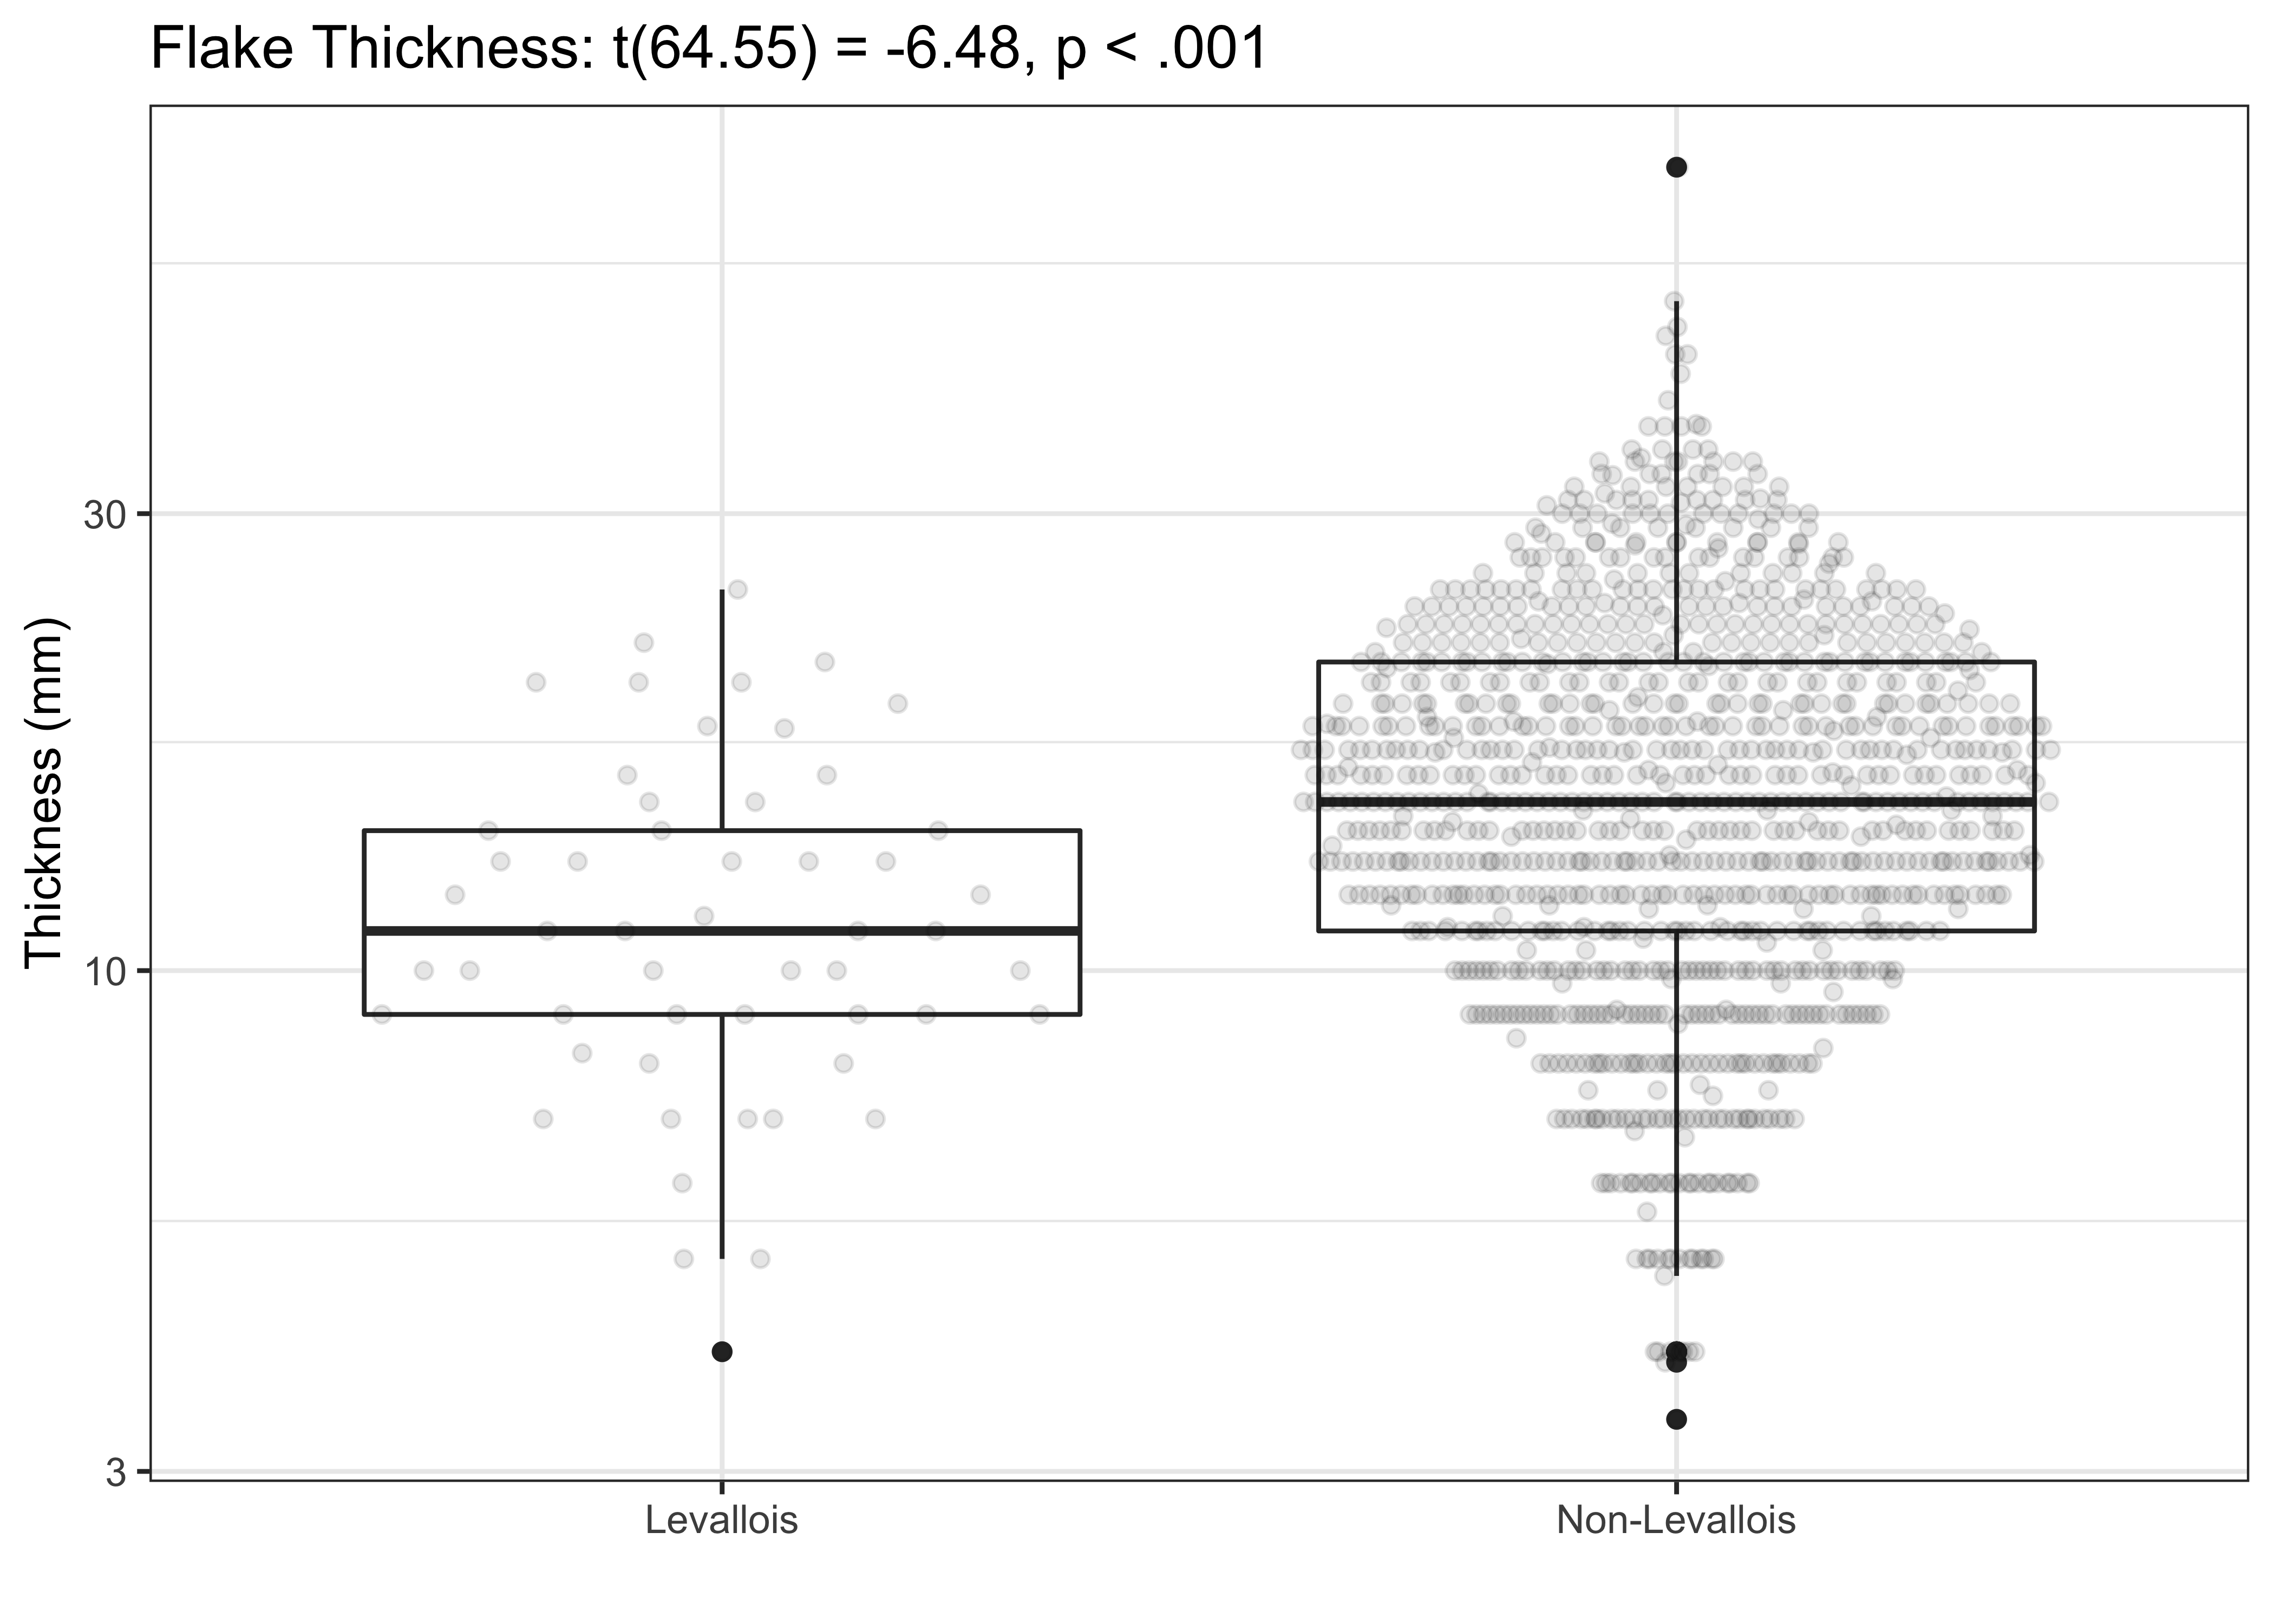
\includegraphics{for_paper_ii_files/figure-latex/unnamed-chunk-7-1.pdf}

\begin{Shaded}
\begin{Highlighting}[]
\KeywordTok{ggplot}\NormalTok{(plain_flakes, }\KeywordTok{aes}\NormalTok{(mass)) }\OperatorTok{+}
\StringTok{  }\KeywordTok{geom_density}\NormalTok{()}
\end{Highlighting}
\end{Shaded}

\includegraphics{for_paper_ii_files/figure-latex/unnamed-chunk-7-2.pdf}

\begin{Shaded}
\begin{Highlighting}[]
\CommentTok{# test is we can discover natural breaks that divide up the flakes?}

\CommentTok{# how many groups should we look for?}
\NormalTok{n <-}\StringTok{ }\DecValTok{5}
\NormalTok{natural_breaks <-}\StringTok{ }\KeywordTok{classIntervals}\NormalTok{(plain_flakes}\OperatorTok{$}\NormalTok{mass, }\DataTypeTok{n =}\NormalTok{ n, }
                                 \DataTypeTok{style =} \StringTok{"jenks"}\NormalTok{, }\DataTypeTok{dataPrecision =} \DecValTok{2}\NormalTok{)}
\CommentTok{# plot the breaks}
\KeywordTok{ggplot}\NormalTok{(plain_flakes, }\KeywordTok{aes}\NormalTok{(mass)) }\OperatorTok{+}
\StringTok{  }\KeywordTok{geom_density}\NormalTok{(}\DataTypeTok{colour =} \StringTok{"blue"}\NormalTok{) }\OperatorTok{+}
\StringTok{  }\KeywordTok{geom_vline}\NormalTok{(}\DataTypeTok{xintercept =}\NormalTok{ natural_breaks}\OperatorTok{$}\NormalTok{brks, }\DataTypeTok{colour =} \StringTok{"red"}\NormalTok{)}
\end{Highlighting}
\end{Shaded}

\includegraphics{for_paper_ii_files/figure-latex/unnamed-chunk-7-3.pdf}

\begin{Shaded}
\begin{Highlighting}[]
\CommentTok{# create a df}
\NormalTok{plain_flakes}\OperatorTok{$}\NormalTok{mass_group <-}\StringTok{ }\KeywordTok{cut}\NormalTok{(plain_flakes}\OperatorTok{$}\NormalTok{mass, }
                               \DataTypeTok{breaks =} \KeywordTok{c}\NormalTok{(}\DecValTok{0}\NormalTok{, natural_breaks}\OperatorTok{$}\NormalTok{brks[}\OperatorTok{-}\DecValTok{1}\NormalTok{]),}
                               \DataTypeTok{labels =} \DecValTok{1}\OperatorTok{:}\NormalTok{(}\KeywordTok{length}\NormalTok{(natural_breaks}\OperatorTok{$}\NormalTok{brks)}\OperatorTok{-}\DecValTok{1}\NormalTok{))}
\CommentTok{# remove flakes not in a group}
\NormalTok{plain_flakes <-}\StringTok{ }\NormalTok{plain_flakes[}\OperatorTok{!}\KeywordTok{is.na}\NormalTok{(plain_flakes}\OperatorTok{$}\NormalTok{mass_group), ]}

\CommentTok{# plot the groups}
\KeywordTok{ggplot}\NormalTok{(plain_flakes, }\KeywordTok{aes}\NormalTok{(mass_group, mass)) }\OperatorTok{+}
\StringTok{  }\KeywordTok{geom_boxplot}\NormalTok{() }\OperatorTok{+}
\StringTok{  }\KeywordTok{geom_jitter}\NormalTok{(}\DataTypeTok{alpha =} \FloatTok{0.1}\NormalTok{) }\OperatorTok{+}
\StringTok{  }\KeywordTok{theme_bw}\NormalTok{()}
\end{Highlighting}
\end{Shaded}

\includegraphics{for_paper_ii_files/figure-latex/unnamed-chunk-7-4.pdf}

\begin{Shaded}
\begin{Highlighting}[]
\CommentTok{# explore variation in thickness in these groups}
\NormalTok{thick_plot <-}\StringTok{ }\KeywordTok{ggplot}\NormalTok{(plain_flakes) }\OperatorTok{+}
\StringTok{  }\KeywordTok{geom_density}\NormalTok{(}\KeywordTok{aes}\NormalTok{(}\StringTok{`}\DataTypeTok{Thickness_25%max}\StringTok{`}\NormalTok{), }\DataTypeTok{colour =} \StringTok{"red"}\NormalTok{, }\DataTypeTok{alpha =} \FloatTok{0.3}\NormalTok{) }\OperatorTok{+}
\StringTok{  }\KeywordTok{geom_density}\NormalTok{(}\KeywordTok{aes}\NormalTok{(}\StringTok{`}\DataTypeTok{Thickness_50%max}\StringTok{`}\NormalTok{), }\DataTypeTok{colour =} \StringTok{"green"}\NormalTok{, }\DataTypeTok{alpha =} \FloatTok{0.3}\NormalTok{) }\OperatorTok{+}
\StringTok{  }\KeywordTok{geom_density}\NormalTok{(}\KeywordTok{aes}\NormalTok{(}\StringTok{`}\DataTypeTok{Thickness_75%max}\StringTok{`}\NormalTok{), }\DataTypeTok{colour =} \StringTok{"blue"}\NormalTok{, }\DataTypeTok{alpha =} \FloatTok{0.3}\NormalTok{) }\OperatorTok{+}
\StringTok{  }\KeywordTok{xlab}\NormalTok{(}\StringTok{"Thickness (mm)"}\NormalTok{) }

\NormalTok{thick_plot }
\end{Highlighting}
\end{Shaded}

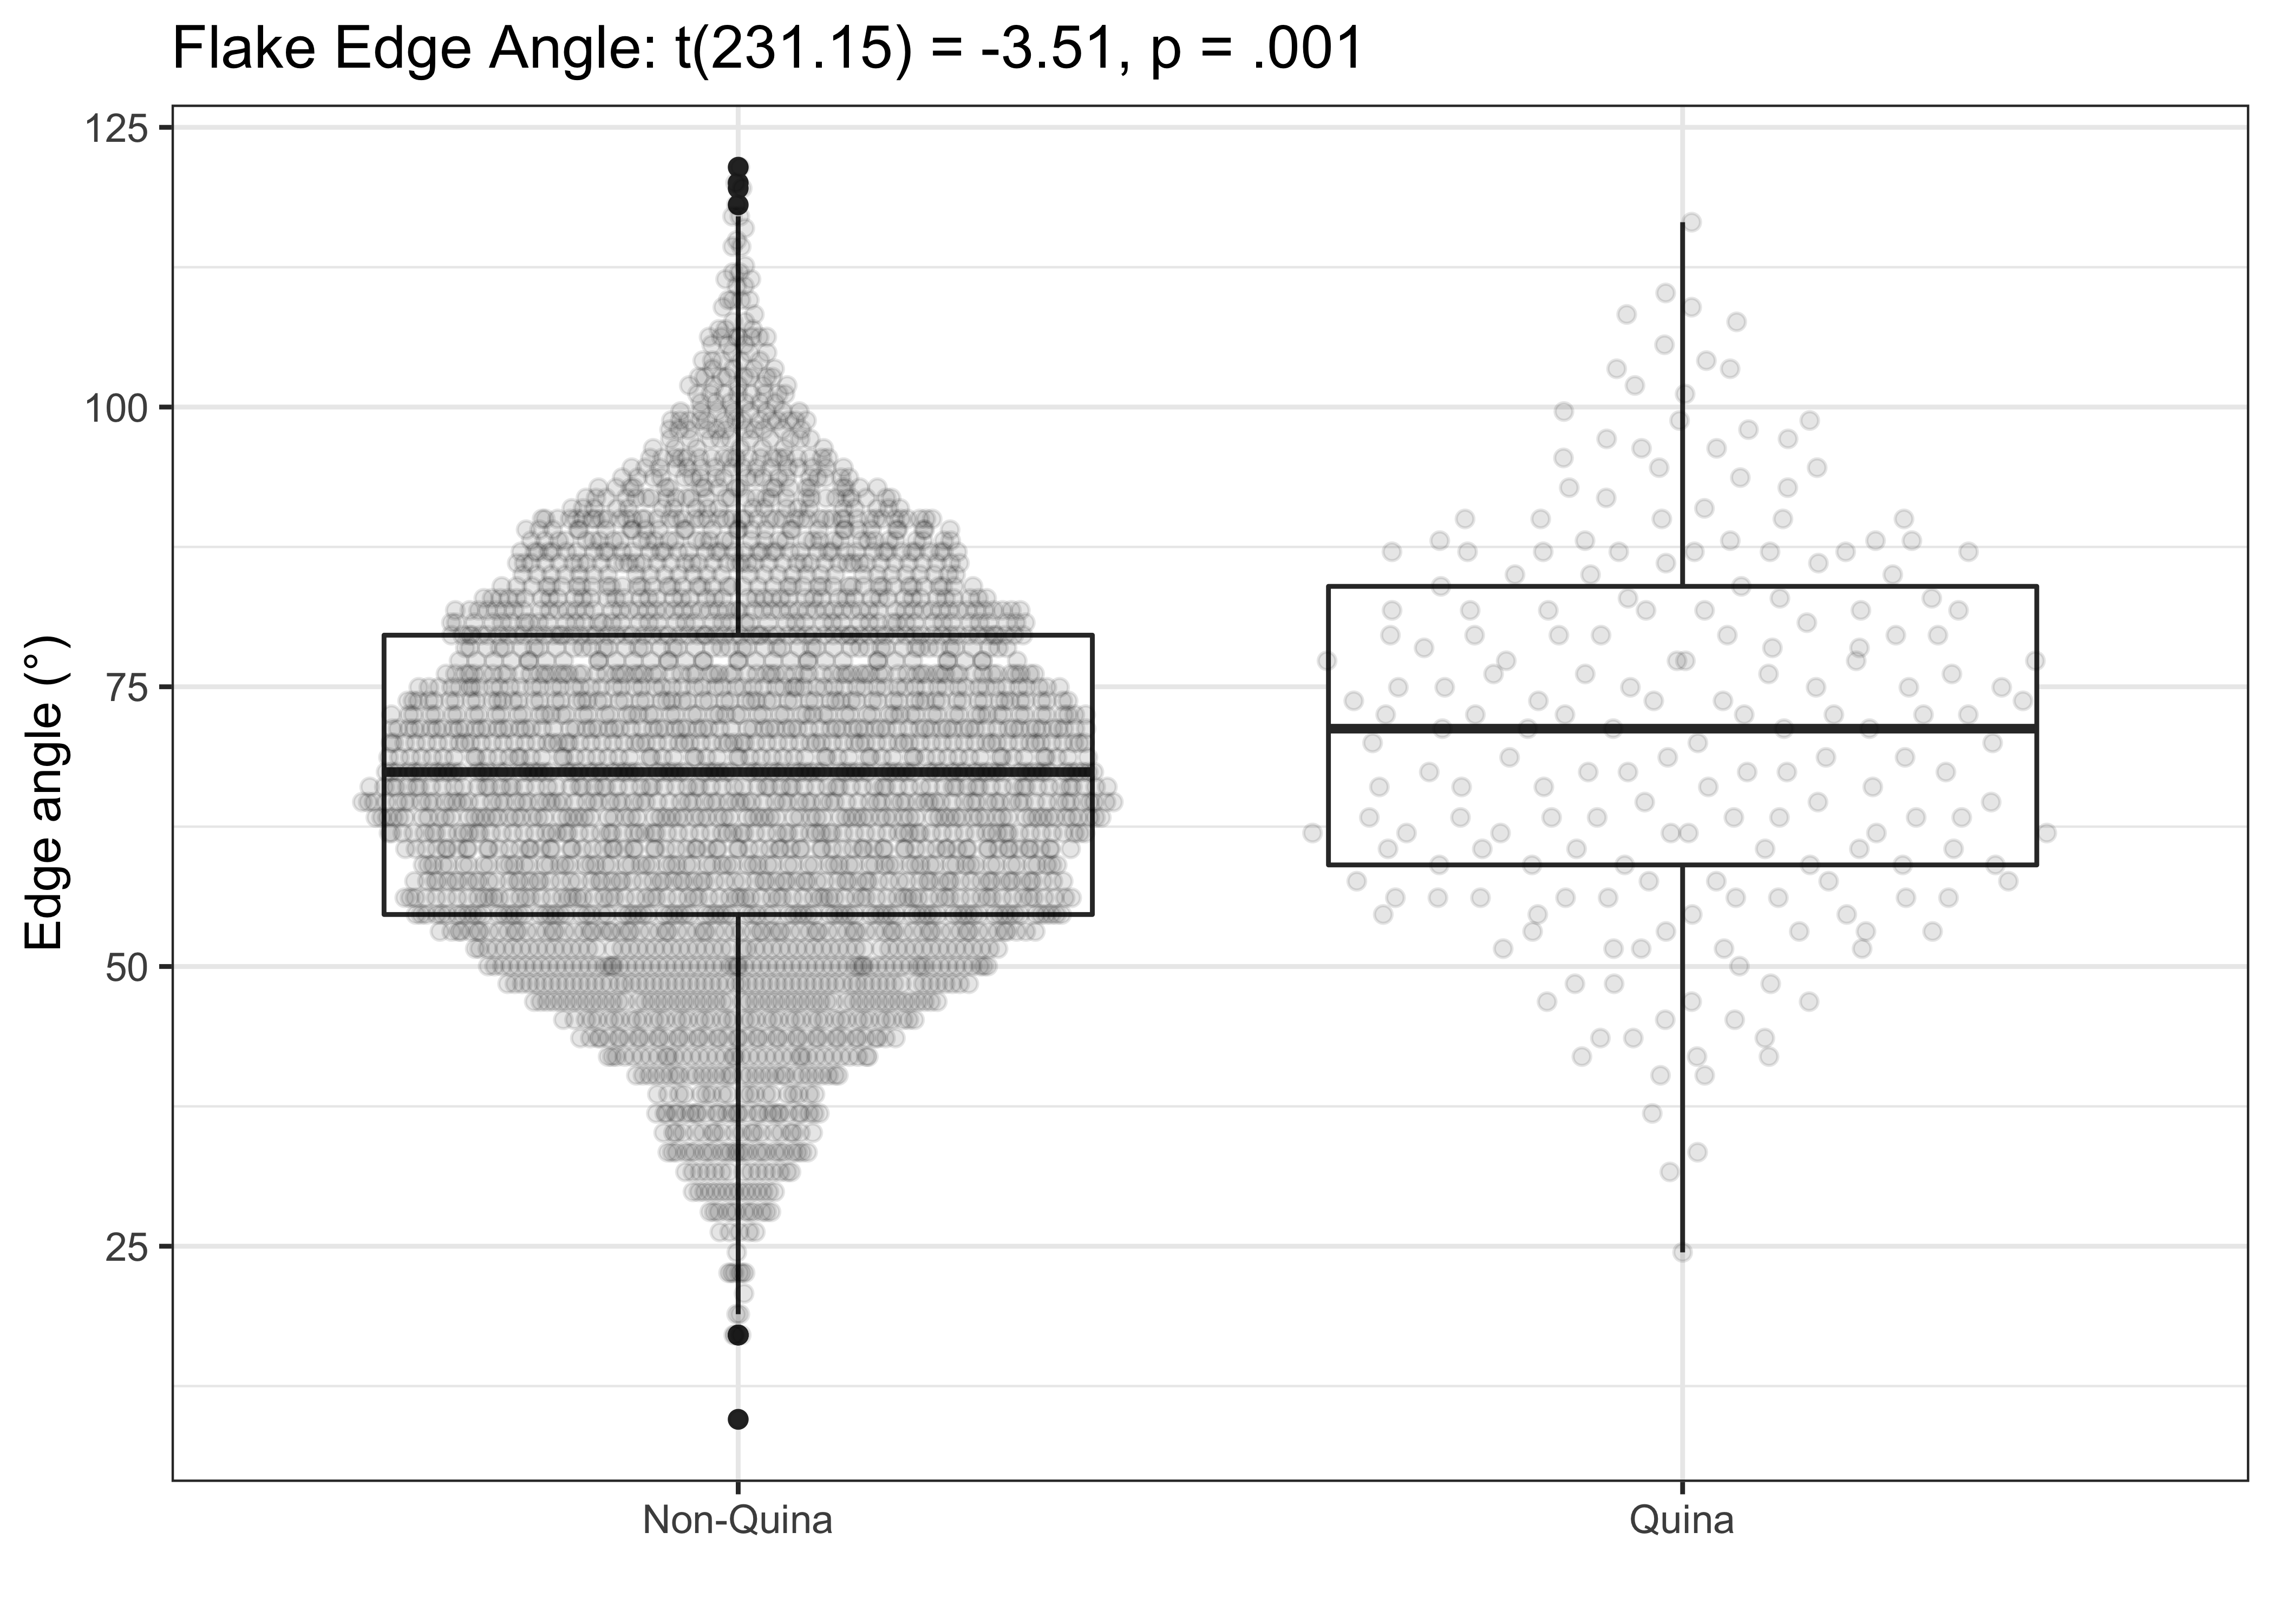
\includegraphics{for_paper_ii_files/figure-latex/unnamed-chunk-8-1.pdf}

\begin{Shaded}
\begin{Highlighting}[]
\CommentTok{# by size class that we identified earlier}
\NormalTok{thick_plot }\OperatorTok{+}
\StringTok{  }\KeywordTok{facet_wrap}\NormalTok{(}\OperatorTok{~}\StringTok{ }\NormalTok{mass_group, }\DataTypeTok{ncol =} \DecValTok{1}\NormalTok{)}
\end{Highlighting}
\end{Shaded}

\includegraphics{for_paper_ii_files/figure-latex/unnamed-chunk-8-2.pdf}

\begin{Shaded}
\begin{Highlighting}[]
\CommentTok{# Lycett and Eren found out the thickness is more evenly distributed and less variable across preferential Levallois flakes. So , let's get the CV values for thickness for each group}
\NormalTok{CV <-}\StringTok{ }\ControlFlowTok{function}\NormalTok{(the_vector)\{}
\NormalTok{  mean_ <-}\StringTok{ }\KeywordTok{mean}\NormalTok{(the_vector, }\DataTypeTok{na.rm =} \OtherTok{TRUE}\NormalTok{)}
\NormalTok{  sd_ <-}\StringTok{ }\KeywordTok{sd}\NormalTok{(the_vector, }\DataTypeTok{na.rm =} \OtherTok{TRUE}\NormalTok{)}
\NormalTok{  cv <-}\StringTok{ }\NormalTok{(sd_}\OperatorTok{/}\NormalTok{mean_)}\OperatorTok{*}\DecValTok{100}
  \KeywordTok{round}\NormalTok{(cv, }\DecValTok{3}\NormalTok{)}
\NormalTok{\}}


\NormalTok{plain_flakes }\OperatorTok\StringTok{ }
\StringTok{  }\KeywordTok{group_by}\NormalTok{(mass_group) }\OperatorTok\StringTok{ }
\StringTok{  }\NormalTok{dplyr}\OperatorTok{::}\KeywordTok{summarise}\NormalTok{(}\DataTypeTok{cv_25_thick =} \KeywordTok{CV}\NormalTok{(}\StringTok{`}\DataTypeTok{Thickness_25%max}\StringTok{`}\NormalTok{),}
                   \DataTypeTok{cv_50_thick =} \KeywordTok{CV}\NormalTok{(}\StringTok{`}\DataTypeTok{Thickness_50%max}\StringTok{`}\NormalTok{),}
                   \DataTypeTok{cv_75_thick =} \KeywordTok{CV}\NormalTok{(}\StringTok{`}\DataTypeTok{Thickness_75%max}\StringTok{`}\NormalTok{),}
                   \DataTypeTok{cv_25_width =} \KeywordTok{CV}\NormalTok{(}\StringTok{`}\DataTypeTok{Width_25%max}\StringTok{`}\NormalTok{), }
                   \DataTypeTok{cv_50_width =} \KeywordTok{CV}\NormalTok{(}\StringTok{`}\DataTypeTok{Width_50%max}\StringTok{`}\NormalTok{),}
                   \DataTypeTok{cv_75_width =} \KeywordTok{CV}\NormalTok{(}\StringTok{`}\DataTypeTok{Width_75%max}\StringTok{`}\NormalTok{), }
                   \DataTypeTok{n =} \KeywordTok{n}\NormalTok{()) }
\end{Highlighting}
\end{Shaded}

\begin{verbatim}
## # A tibble: 5 x 8
##   mass_group cv_25_thick cv_50_thick cv_75_thick cv_25_width cv_50_width
##   <fct>            <dbl>       <dbl>       <dbl>       <dbl>       <dbl>
## 1 1                 47.7        46.5        49.8        35.3       34.4 
## 2 2                 26.7        21.5        24.0        17.5       17.2 
## 3 3                 20.9        12.9        23.4        23.8        9.65
## 4 4                 11.1        32.1        26.4        17.7       10.6 
## 5 5                 NA          NA          NA          NA         NA   
## # ... with 2 more variables: cv_75_width <dbl>, n <int>
\end{verbatim}

\begin{Shaded}
\begin{Highlighting}[]
\CommentTok{# calculate the edge angle}

\NormalTok{edge_angle_}\DecValTok{2}\NormalTok{ <-}\StringTok{ }\NormalTok{edge_angle}

\NormalTok{edge_angle_}\DecValTok{2}\NormalTok{[, }\DecValTok{2}\OperatorTok{:}\NormalTok{(}\KeywordTok{ncol}\NormalTok{(edge_angle_}\DecValTok{2}\NormalTok{)}\OperatorTok{-}\DecValTok{1}\NormalTok{)] <-}\StringTok{ }\KeywordTok{atan}\NormalTok{(edge_angle[, }\DecValTok{2}\OperatorTok{:}\NormalTok{(}\KeywordTok{ncol}\NormalTok{(edge_angle_}\DecValTok{2}\NormalTok{)}\OperatorTok{-}\DecValTok{1}\NormalTok{)]}\OperatorTok{/}\DecValTok{2}\OperatorTok{/}\DecValTok{3}\NormalTok{)}\OperatorTok{/}\NormalTok{pi}\OperatorTok{*}\DecValTok{180}\OperatorTok{*}\DecValTok{2}



\NormalTok{df_angle <-}\StringTok{ }\KeywordTok{melt}\NormalTok{(edge_angle_}\DecValTok{2}\NormalTok{)}
\end{Highlighting}
\end{Shaded}

\begin{verbatim}
## Using number, X__1 as id variables
\end{verbatim}

\begin{Shaded}
\begin{Highlighting}[]
\CommentTok{# plot the angles }
\KeywordTok{ggplot}\NormalTok{(df_angle, }\KeywordTok{aes}\NormalTok{(}\DataTypeTok{x =}\NormalTok{ value, }\DataTypeTok{col =}\NormalTok{ variable)) }\OperatorTok{+}\StringTok{ }\KeywordTok{geom_density}\NormalTok{() }\OperatorTok{+}\StringTok{ }\KeywordTok{theme_bw}\NormalTok{()}
\end{Highlighting}
\end{Shaded}

\begin{verbatim}
## Warning: Removed 5480 rows containing non-finite values (stat_density).
\end{verbatim}

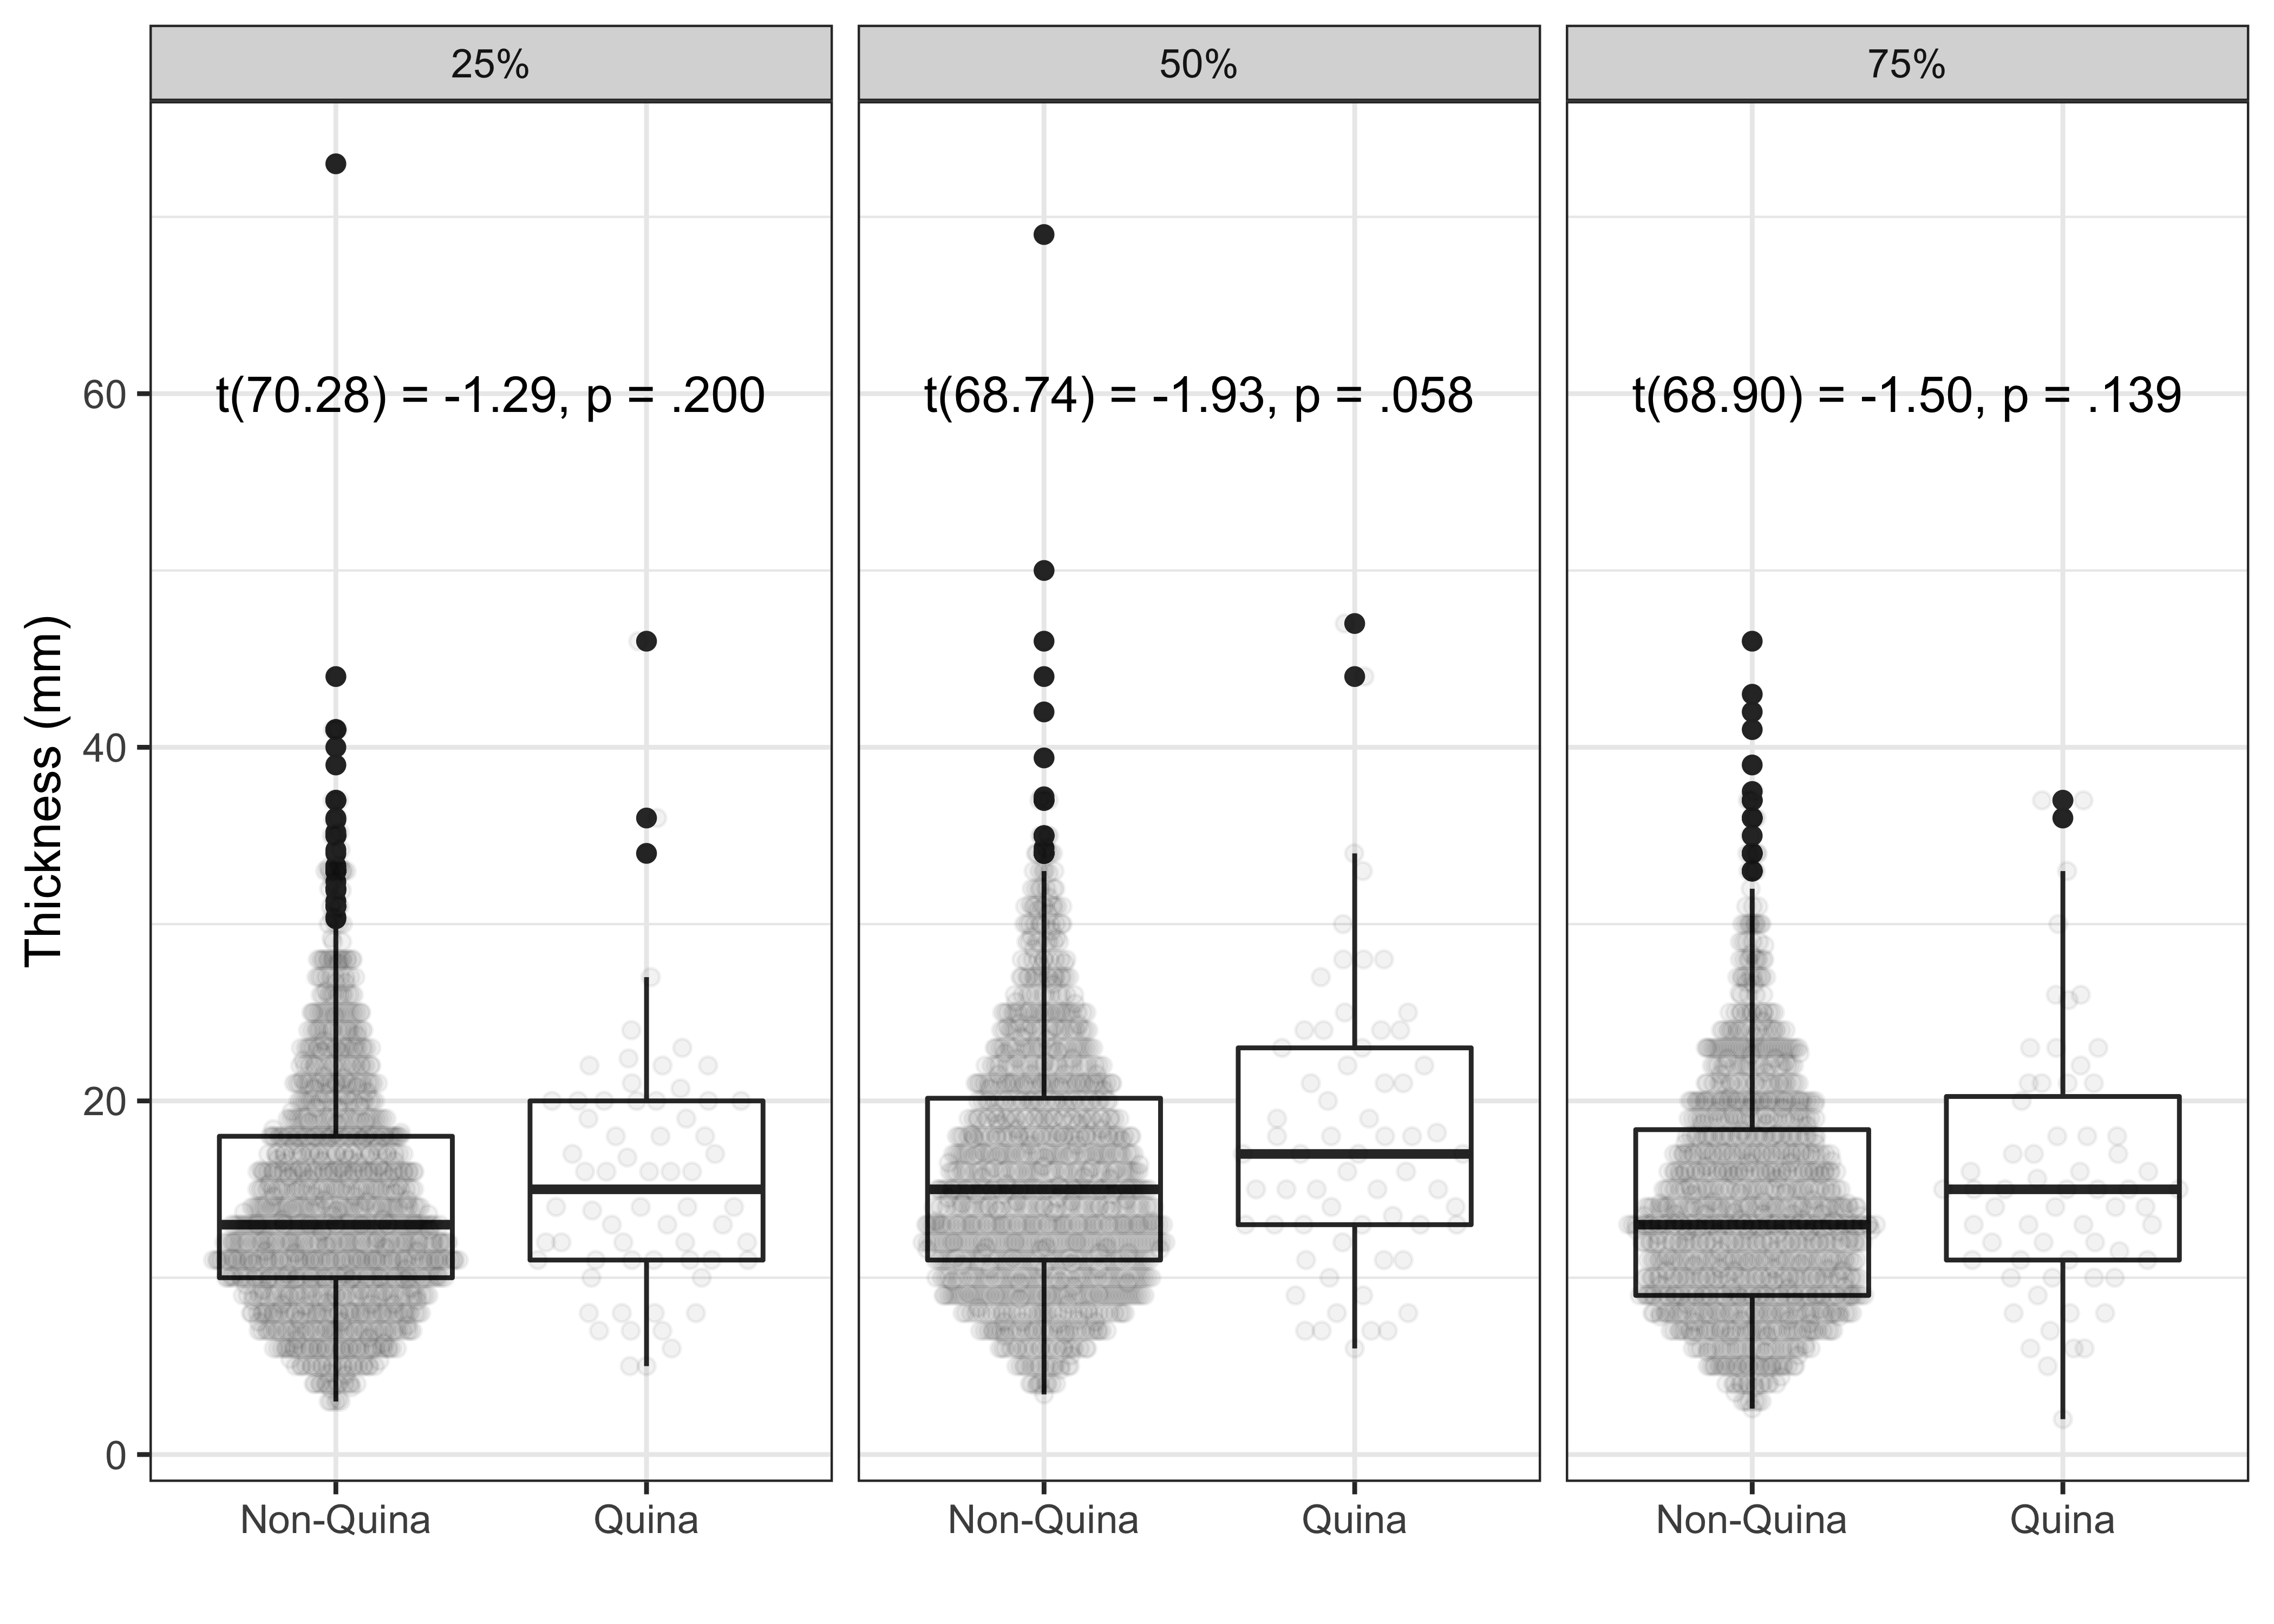
\includegraphics{for_paper_ii_files/figure-latex/unnamed-chunk-9-1.pdf}

\begin{Shaded}
\begin{Highlighting}[]
\NormalTok{## find quina and compare their angles.}

\NormalTok{quina_id <-}\StringTok{ }\NormalTok{flakes}\OperatorTok{$}\NormalTok{number[}\KeywordTok{which}\NormalTok{(flakes}\OperatorTok{$}\NormalTok{type3 }\OperatorTok{==}\StringTok{ "quina"}\NormalTok{)]}

\NormalTok{df_angle}\OperatorTok{$}\NormalTok{quina <-}\StringTok{ }\KeywordTok{ifelse}\NormalTok{(df_angle}\OperatorTok{$}\NormalTok{number }\OperatorTok\StringTok{ }\NormalTok{quina_id, }\StringTok{"quina"}\NormalTok{, }\StringTok{"no"}\NormalTok{)}

\KeywordTok{ggplot}\NormalTok{(df_angle, }\KeywordTok{aes}\NormalTok{(}\DataTypeTok{x =}\NormalTok{ value, }\DataTypeTok{col =}\NormalTok{ quina)) }\OperatorTok{+}\StringTok{ }\KeywordTok{geom_density}\NormalTok{() }\OperatorTok{+}\StringTok{ }\KeywordTok{theme_bw}\NormalTok{()}
\end{Highlighting}
\end{Shaded}

\begin{verbatim}
## Warning: Removed 5480 rows containing non-finite values (stat_density).
\end{verbatim}

\includegraphics{for_paper_ii_files/figure-latex/unnamed-chunk-9-2.pdf}

\begin{Shaded}
\begin{Highlighting}[]
\KeywordTok{ggplot}\NormalTok{(df_angle, }\KeywordTok{aes}\NormalTok{(}\DataTypeTok{x =}\NormalTok{ value, }\DataTypeTok{col =}\NormalTok{ variable)) }\OperatorTok{+}\StringTok{ }\KeywordTok{geom_density}\NormalTok{() }\OperatorTok{+}\StringTok{ }\KeywordTok{theme_bw}\NormalTok{() }\OperatorTok{+}\StringTok{ }\KeywordTok{facet_wrap}\NormalTok{(}\OperatorTok{~}\NormalTok{quina)}
\end{Highlighting}
\end{Shaded}

\begin{verbatim}
## Warning: Removed 5480 rows containing non-finite values (stat_density).
\end{verbatim}

\includegraphics{for_paper_ii_files/figure-latex/unnamed-chunk-9-3.pdf}

\begin{Shaded}
\begin{Highlighting}[]
\NormalTok{## compare thickness of quina and other}

\NormalTok{df_thick <-}\StringTok{ }\KeywordTok{melt}\NormalTok{(flakes[, }\KeywordTok{c}\NormalTok{(}\StringTok{"number"}\NormalTok{, }\StringTok{"Thickness_25%max"}\NormalTok{, }\StringTok{"Thickness_50%max"}\NormalTok{, }\StringTok{"Thickness_75%max"}\NormalTok{)])}
\end{Highlighting}
\end{Shaded}

\begin{verbatim}
## Using number as id variables
\end{verbatim}

\begin{Shaded}
\begin{Highlighting}[]
\NormalTok{df_thick}\OperatorTok{$}\NormalTok{quina <-}\StringTok{ }\KeywordTok{ifelse}\NormalTok{(df_thick}\OperatorTok{$}\NormalTok{number }\OperatorTok\StringTok{ }\NormalTok{quina_id, }\StringTok{"quina"}\NormalTok{, }\StringTok{"no"}\NormalTok{)}

\KeywordTok{ggplot}\NormalTok{(df_thick, }\KeywordTok{aes}\NormalTok{(}\DataTypeTok{x =}\NormalTok{ value, }\DataTypeTok{col =}\NormalTok{ quina)) }\OperatorTok{+}\StringTok{ }\KeywordTok{geom_density}\NormalTok{() }\OperatorTok{+}\StringTok{ }\KeywordTok{theme_bw}\NormalTok{() }\OperatorTok{+}\StringTok{ }\KeywordTok{facet_wrap}\NormalTok{(}\OperatorTok{~}\NormalTok{variable)}
\end{Highlighting}
\end{Shaded}

\begin{verbatim}
## Warning: Removed 96 rows containing non-finite values (stat_density).
\end{verbatim}

\includegraphics{for_paper_ii_files/figure-latex/unnamed-chunk-9-4.pdf}

\begin{Shaded}
\begin{Highlighting}[]
\CommentTok{# plot the thickness of 50% max}
\KeywordTok{ggplot}\NormalTok{(df_thick[df_thick}\OperatorTok{$}\NormalTok{variable }\OperatorTok{==}\StringTok{"Thickness_50%max"}\NormalTok{, ], }\KeywordTok{aes}\NormalTok{(quina, value)) }\OperatorTok{+}
\StringTok{  }\KeywordTok{geom_boxplot}\NormalTok{() }\OperatorTok{+}\StringTok{ }\KeywordTok{theme_bw}\NormalTok{()}
\end{Highlighting}
\end{Shaded}

\begin{verbatim}
## Warning: Removed 32 rows containing non-finite values (stat_boxplot).
\end{verbatim}

\includegraphics{for_paper_ii_files/figure-latex/unnamed-chunk-9-5.pdf}

\begin{Shaded}
\begin{Highlighting}[]
\NormalTok{## count the number of shapes of edges.}

\NormalTok{edge_shapes <-}\StringTok{ }\KeywordTok{unlist}\NormalTok{(}\KeywordTok{strsplit}\NormalTok{(retouch}\OperatorTok{$}\StringTok{`}\DataTypeTok{edge shape}\StringTok{`}\NormalTok{, }\StringTok{","}\NormalTok{))}

\KeywordTok{data.frame}\NormalTok{(}\KeywordTok{table}\NormalTok{(edge_shapes)) }\OperatorTok\StringTok{ }
\KeywordTok{ggplot}\NormalTok{(}\KeywordTok{aes}\NormalTok{(}\DataTypeTok{x =} \KeywordTok{reorder}\NormalTok{(edge_shapes, Freq), }\DataTypeTok{y =}\NormalTok{ Freq)) }\OperatorTok{+}
\StringTok{    }\KeywordTok{geom_bar}\NormalTok{(}\DataTypeTok{stat =} \StringTok{"identity"}\NormalTok{) }\OperatorTok{+}
\StringTok{    }\KeywordTok{ylab}\NormalTok{(}\StringTok{"n"}\NormalTok{) }\OperatorTok{+}
\StringTok{    }\KeywordTok{xlab}\NormalTok{(}\StringTok{"Edge type"}\NormalTok{) }\OperatorTok{+}\StringTok{ }
\StringTok{    }\KeywordTok{theme_bw}\NormalTok{() }\OperatorTok{+}
\StringTok{    }\KeywordTok{theme}\NormalTok{(}\DataTypeTok{axis.text.x =} \KeywordTok{element_text}\NormalTok{(}\DataTypeTok{angle =} \DecValTok{90}\NormalTok{, }\DataTypeTok{hjust =} \DecValTok{1}\NormalTok{, }\DataTypeTok{vjust =} \FloatTok{0.5}\NormalTok{))}
\end{Highlighting}
\end{Shaded}

\includegraphics{for_paper_ii_files/figure-latex/unnamed-chunk-9-6.pdf}

\begin{Shaded}
\begin{Highlighting}[]
\KeywordTok{data.frame}\NormalTok{(}\KeywordTok{table}\NormalTok{(edge_shapes))}
\end{Highlighting}
\end{Shaded}

\begin{verbatim}
##   edge_shapes Freq
## 1         bec    3
## 2       borer   40
## 3         ccv  274
## 4         cvx  395
## 5        dent  134
## 6         end   32
## 7       notch  106
## 8        strt  575
\end{verbatim}

\begin{Shaded}
\begin{Highlighting}[]
\NormalTok{## number of layers}

\KeywordTok{f}\NormalTok{(retouch, }\StringTok{'number of layers'}\NormalTok{)}
\end{Highlighting}
\end{Shaded}

\includegraphics{for_paper_ii_files/figure-latex/unnamed-chunk-9-7.pdf}

\begin{Shaded}
\begin{Highlighting}[]
\NormalTok{## number of edges}

\KeywordTok{f}\NormalTok{(retouch, }\StringTok{'number of edge'}\NormalTok{)}
\end{Highlighting}
\end{Shaded}

\includegraphics{for_paper_ii_files/figure-latex/unnamed-chunk-9-8.pdf}

\begin{Shaded}
\begin{Highlighting}[]
\NormalTok{## number of layers for each number of eadge}

\NormalTok{df_layer_edge <-}\StringTok{ }\KeywordTok{melt}\NormalTok{(retouch[, }\DecValTok{1}\OperatorTok{:}\DecValTok{3}\NormalTok{])}
\end{Highlighting}
\end{Shaded}

\begin{verbatim}
## Using number as id variables
\end{verbatim}

\begin{Shaded}
\begin{Highlighting}[]
 \KeywordTok{data.frame}\NormalTok{(}\KeywordTok{table}\NormalTok{(retouch[,}\DecValTok{2}\OperatorTok{:}\DecValTok{3}\NormalTok{])) }\OperatorTok\StringTok{ }
\StringTok{    }\KeywordTok{ggplot}\NormalTok{(}\KeywordTok{aes}\NormalTok{(}\DataTypeTok{x =} \KeywordTok{reorder}\NormalTok{(number.of.layers, Freq), }\DataTypeTok{y =}\NormalTok{ Freq)) }\OperatorTok{+}
\StringTok{    }\KeywordTok{geom_bar}\NormalTok{(}\DataTypeTok{stat =} \StringTok{"identity"}\NormalTok{) }\OperatorTok{+}
\StringTok{    }\KeywordTok{ylab}\NormalTok{(}\StringTok{"n"}\NormalTok{) }\OperatorTok{+}
\StringTok{    }\KeywordTok{xlab}\NormalTok{(}\StringTok{"number of layers"}\NormalTok{) }\OperatorTok{+}\StringTok{ }
\StringTok{    }\KeywordTok{theme_bw}\NormalTok{() }\OperatorTok{+}
\StringTok{    }\KeywordTok{theme}\NormalTok{(}\DataTypeTok{axis.text.x =} \KeywordTok{element_text}\NormalTok{(}\DataTypeTok{angle =} \DecValTok{90}\NormalTok{, }\DataTypeTok{hjust =} \DecValTok{1}\NormalTok{, }\DataTypeTok{vjust =} \FloatTok{0.5}\NormalTok{)) }\OperatorTok{+}
\StringTok{    }\KeywordTok{facet_wrap}\NormalTok{(}\OperatorTok{~}\NormalTok{number.of.edge)}
\end{Highlighting}
\end{Shaded}

\includegraphics{for_paper_ii_files/figure-latex/unnamed-chunk-9-9.pdf}

\begin{Shaded}
\begin{Highlighting}[]
\CommentTok{# scar number and direction}

\NormalTok{## count how many scars from each direction}

\KeywordTok{table}\NormalTok{(}\KeywordTok{unlist}\NormalTok{(scar_dir[,}\DecValTok{2}\OperatorTok{:}\DecValTok{8}\NormalTok{]))}
\end{Highlighting}
\end{Shaded}

\begin{verbatim}
## 
##   0   1   2   3   4   5   6   7   8 
##  85 221 168 109  73  68  61  71 138
\end{verbatim}

\begin{Shaded}
\begin{Highlighting}[]
\NormalTok{## calculate GIUR}

\NormalTok{df_giur <-}\StringTok{ }\NormalTok{retouch[, }\KeywordTok{c}\NormalTok{(}\DecValTok{1}\NormalTok{,}\DecValTok{8}\NormalTok{,}\DecValTok{10}\NormalTok{,}\DecValTok{12}\NormalTok{,}\DecValTok{14}\NormalTok{,}\DecValTok{16}\NormalTok{,}\DecValTok{18}\NormalTok{,}\DecValTok{20}\NormalTok{,}\DecValTok{22}\NormalTok{)]}

\NormalTok{df_giur[, }\OperatorTok{-}\DecValTok{1}\NormalTok{] <-}\StringTok{ }\NormalTok{df_giur[, }\OperatorTok{-}\DecValTok{1}\NormalTok{] }\OperatorTok{/}\StringTok{ }\NormalTok{retouch[, }\KeywordTok{c}\NormalTok{(}\DecValTok{9}\NormalTok{,}\DecValTok{11}\NormalTok{,}\DecValTok{13}\NormalTok{,}\DecValTok{15}\NormalTok{,}\DecValTok{17}\NormalTok{,}\DecValTok{19}\NormalTok{,}\DecValTok{21}\NormalTok{,}\DecValTok{23}\NormalTok{)]}

\NormalTok{df_giur_clustered <-}\StringTok{ }\KeywordTok{left_join}\NormalTok{(df_giur, flakes_clustered[, }\KeywordTok{c}\NormalTok{(}\StringTok{"number"}\NormalTok{, }\StringTok{"cluster"}\NormalTok{)])}
\end{Highlighting}
\end{Shaded}

\begin{verbatim}
## Joining, by = "number"
\end{verbatim}

\begin{Shaded}
\begin{Highlighting}[]
\NormalTok{df_giur_clustered_melt <-}\StringTok{ }\KeywordTok{melt}\NormalTok{(df_giur_clustered[,}\OperatorTok{-}\DecValTok{1}\NormalTok{], }\DataTypeTok{id.vars =} \StringTok{"cluster"}\NormalTok{)}

\NormalTok{## compare GIUR for different mass categories}

\KeywordTok{ggplot}\NormalTok{(}\KeywordTok{na.omit}\NormalTok{(df_giur_clustered_melt[df_giur_clustered_melt}\OperatorTok{$}\NormalTok{value }\OperatorTok{<=}\DecValTok{1}\NormalTok{,]), }\KeywordTok{aes}\NormalTok{(value)) }\OperatorTok{+}
\StringTok{  }\KeywordTok{geom_histogram}\NormalTok{() }\OperatorTok{+}\StringTok{ }\KeywordTok{facet_wrap}\NormalTok{(}\OperatorTok{~}\NormalTok{cluster)}
\end{Highlighting}
\end{Shaded}

\begin{verbatim}
## `stat_bin()` using `bins = 30`. Pick better value with `binwidth`.
\end{verbatim}

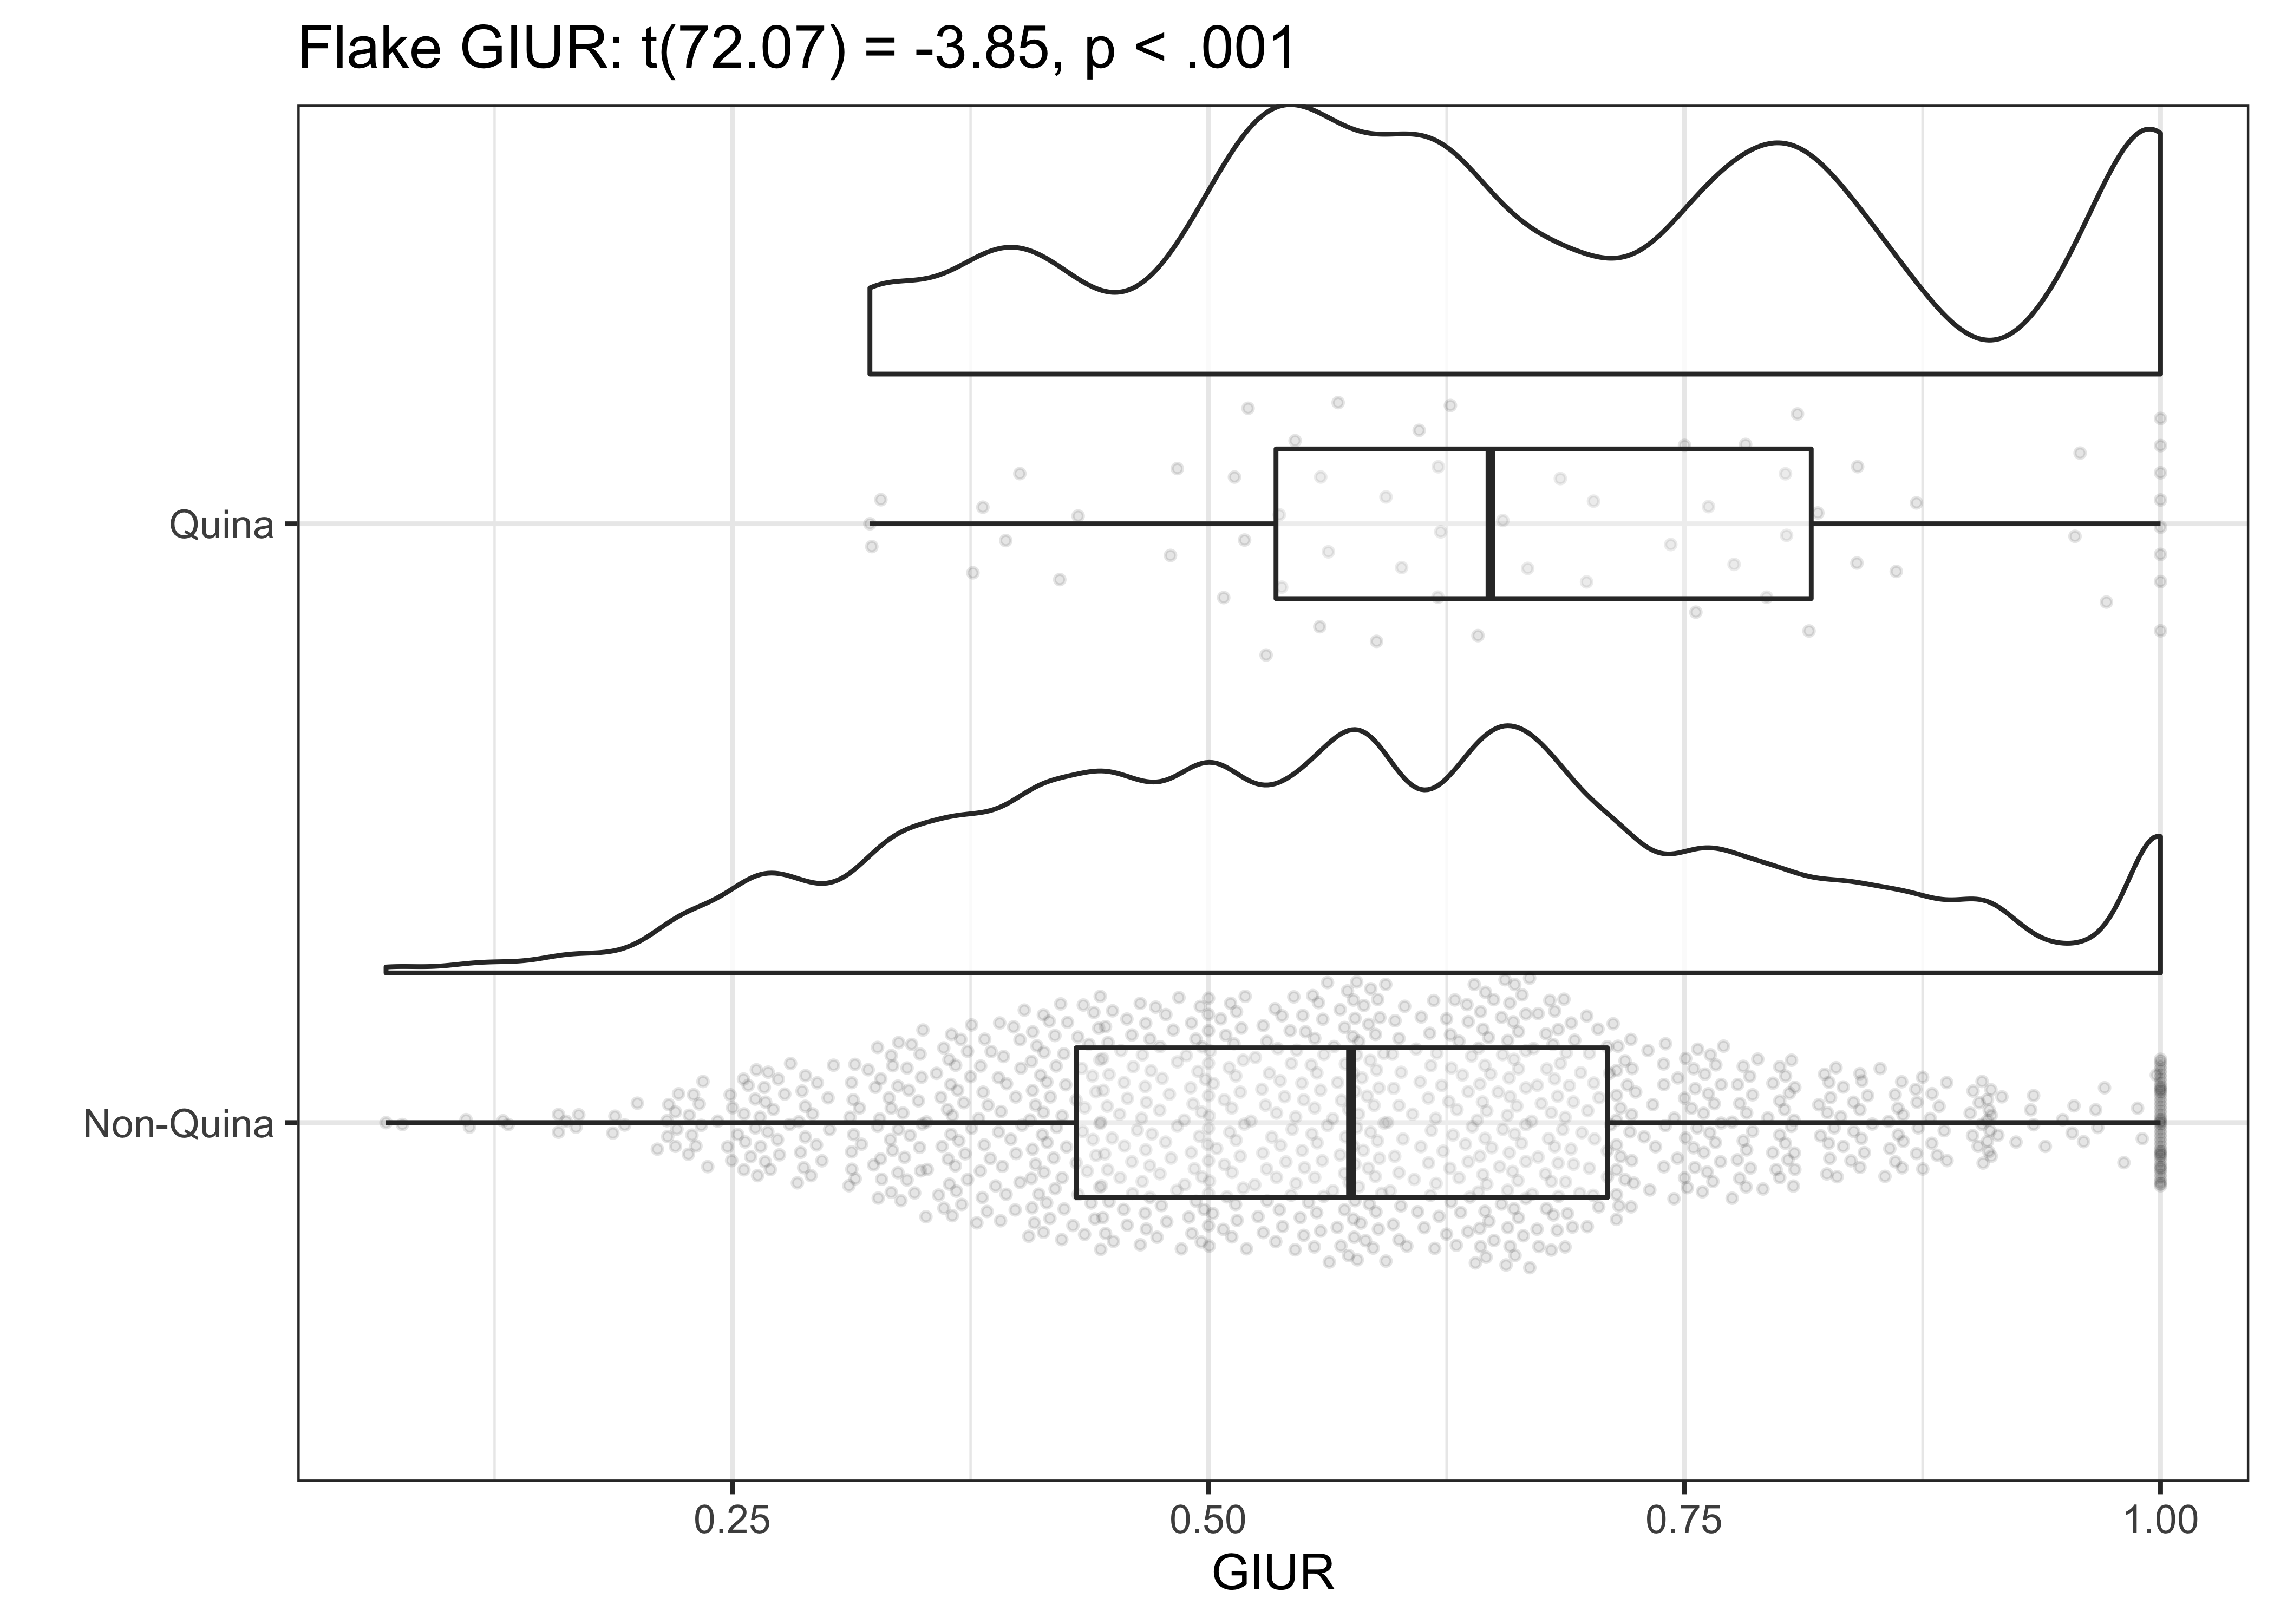
\includegraphics{for_paper_ii_files/figure-latex/unnamed-chunk-10-1.pdf}

\begin{Shaded}
\begin{Highlighting}[]
\NormalTok{## calculate the median GIUR for each group}

\KeywordTok{tapply}\NormalTok{(df_giur_clustered_melt}\OperatorTok{$}\NormalTok{value, df_giur_clustered_melt}\OperatorTok{$}\NormalTok{cluster, median, }\DataTypeTok{na.rm=}\OtherTok{TRUE}\NormalTok{)}
\end{Highlighting}
\end{Shaded}

\begin{verbatim}
##         1         2         3         4         5 
## 0.5963639 0.5433333 0.4739884 0.4400000 0.5151515
\end{verbatim}

\begin{Shaded}
\begin{Highlighting}[]
\CommentTok{# Invasiveness index}

\NormalTok{df_invasive <-}\StringTok{ }\NormalTok{retouch[, }\KeywordTok{c}\NormalTok{(}\DecValTok{1}\NormalTok{, }\DecValTok{24}\OperatorTok{:}\DecValTok{39}\NormalTok{)]}

\NormalTok{df_invasive_clustered <-}\StringTok{ }\KeywordTok{left_join}\NormalTok{(df_invasive, flakes_clustered[, }\KeywordTok{c}\NormalTok{(}\StringTok{"number"}\NormalTok{, }\StringTok{"cluster"}\NormalTok{)])}
\end{Highlighting}
\end{Shaded}

\begin{verbatim}
## Joining, by = "number"
\end{verbatim}

\begin{Shaded}
\begin{Highlighting}[]
\NormalTok{df_invasive_clustered_melt <-}\StringTok{ }\KeywordTok{melt}\NormalTok{(df_invasive_clustered[,}\OperatorTok{-}\DecValTok{1}\NormalTok{], }\DataTypeTok{id.vars =} \StringTok{"cluster"}\NormalTok{)}

\NormalTok{invasive_table <-}\StringTok{ }\KeywordTok{as.data.frame}\NormalTok{(}\KeywordTok{table}\NormalTok{(df_invasive_clustered_melt[, }\KeywordTok{c}\NormalTok{(}\StringTok{"cluster"}\NormalTok{, }\StringTok{"value"}\NormalTok{)]))}

\KeywordTok{ggplot}\NormalTok{(invasive_table[invasive_table}\OperatorTok{$}\NormalTok{value }\OperatorTok\StringTok{ }\KeywordTok{c}\NormalTok{(}\FloatTok{0.5}\NormalTok{, }\FloatTok{1.0}\NormalTok{), ], }\KeywordTok{aes}\NormalTok{(}\DataTypeTok{fill=}\NormalTok{value, }\DataTypeTok{y=}\NormalTok{ Freq, }\DataTypeTok{x=}\NormalTok{cluster)) }\OperatorTok{+}\StringTok{ }
\StringTok{    }\KeywordTok{geom_bar}\NormalTok{( }\DataTypeTok{stat=}\StringTok{"identity"}\NormalTok{, }\DataTypeTok{position=}\StringTok{"fill"}\NormalTok{, }\DataTypeTok{width =} \FloatTok{0.6}\NormalTok{) }\OperatorTok{+}\StringTok{ }\KeywordTok{theme_bw}\NormalTok{() }\OperatorTok{+}
\StringTok{    }\KeywordTok{theme}\NormalTok{(}\DataTypeTok{axis.text=}\KeywordTok{element_text}\NormalTok{(}\DataTypeTok{size=}\DecValTok{14}\NormalTok{), }\DataTypeTok{axis.title=}\KeywordTok{element_text}\NormalTok{(}\DataTypeTok{size=}\DecValTok{16}\NormalTok{,}\DataTypeTok{face=}\StringTok{"bold"}\NormalTok{)) }\OperatorTok{+}
\StringTok{    }\KeywordTok{theme}\NormalTok{(}\DataTypeTok{legend.text=}\KeywordTok{element_text}\NormalTok{(}\DataTypeTok{size=}\DecValTok{14}\NormalTok{))}
\end{Highlighting}
\end{Shaded}

\includegraphics{for_paper_ii_files/figure-latex/unnamed-chunk-10-2.pdf}


\end{document}
